\documentclass{article}

% ---------- NeurIPS 2026 style ----------
% Default is the "main" track in double-blind submission mode (anonymous +
% line numbers). To produce a non-anonymous preprint for personal circulation
% or arXiv, swap the line below for:
%     \usepackage[preprint]{neurips_2026}
% For the camera-ready final version (post-acceptance only):
%     \usepackage[main, final]{neurips_2026}
\usepackage[preprint]{neurips_2026}

% ---------- Core packages ----------
\usepackage[utf8]{inputenc}
\usepackage[T1]{fontenc}
\usepackage{graphicx}
\usepackage{amsmath, amssymb, amsthm}
\usepackage{mathtools}
\usepackage{bm}
\usepackage{booktabs}
\usepackage{hyperref}
\usepackage{cleveref}
\usepackage{xcolor}
\usepackage{url}


% ---------- Theorem environments ----------
\theoremstyle{plain}
\newtheorem{theorem}{Theorem}
\newtheorem{proposition}[theorem]{Proposition}
\newtheorem{lemma}[theorem]{Lemma}
\newtheorem{corollary}[theorem]{Corollary}

\theoremstyle{definition}
\newtheorem{definition}[theorem]{Definition}
\newtheorem{assumption}[theorem]{Assumption}

\theoremstyle{remark}
\newtheorem{remark}[theorem]{Remark}

% ---------- Notation macros ----------
\newcommand{\R}{\mathbb{R}}
\newcommand{\E}{\mathbb{E}}
\newcommand{\Prob}{\mathbb{P}}
\newcommand{\Agents}{\mathcal{A}}        % agent set
\newcommand{\Normal}{\mathcal{N}}        % Gaussian distribution
\newcommand{\Obs}{\mathcal{O}}           % observation space
\newcommand{\Rollouts}{\mathcal{B}}      % rollout observation set
\newcommand{\Pairs}{\mathcal{P}}         % set of unordered pairs
\newcommand{\policy}[1]{\pi_{\theta_{#1}}}
\newcommand{\Wass}{W_2}
\newcommand{\SND}{\ensuremath{\mathrm{SND}}}
\newcommand{\SNDG}{\mathrm{SND}_{G}}
\newcommand{\HSE}{\mathrm{HSE}}
\newcommand{\abs}[1]{\left\lvert #1 \right\rvert}
\newcommand{\norm}[1]{\left\lVert #1 \right\rVert}
\newcommand{\ind}{\mathbf{1}}

% ---------- Anonymisation-aware helpers ----------
% \codelocation resolves to "Code will be released upon acceptance."
% in double-blind submission mode, and to the GitHub URL otherwise.
% Driven by the NeurIPS style file's internal \if@anonymous flag.
\makeatletter
\newcommand{\codelocation}{%
  \if@anonymous
    Code will be released upon acceptance (anonymous supplementary
    material accompanies this submission).%
  \else
    Code: \url{https://github.com/codingwithshawnyt/Graph-SND}.%
  \fi
}
\makeatother

% ---------- Title ----------
\title{Scalable System Neural Diversity:\\
Graph-Based Local Aggregation and Sampling-Based Estimation}

% The NeurIPS 2026 style file automatically anonymizes the author block in
% double-blind submission mode. In preprint / final mode the block below is
% rendered as-is.
\author{%
  Shawn Ray \\
  Carnegie Mellon University \\
  \texttt{shawnray@cmu.edu} \\
}

\begin{document}
\maketitle

\begin{abstract}
System Neural Diversity (SND) quantifies behavioral heterogeneity in
multi-agent RL by averaging pairwise Wasserstein distances over all
$\binom{n}{2}$ agent pairs, scaling as $O(n^2)$; its authors flag
sparse-graph generalizations as open. We introduce Graph-SND, a
graph-structured generalization that evaluates pairwise distances only
on the edges of a user-specified graph $G$ and aggregates them as a
normalized weighted mean. The construction recovers SND exactly when
$G$ is complete and admits two interpretations selected by $G$: a
\emph{fixed} $G$ encoding task-relevant interaction structure yields a
localized diversity measure at cost $O(|E|)$; a \emph{random} $G$ with
Horvitz--Thompson weights yields an unbiased estimator of full SND
with a Hoeffding-type $O(1/\sqrt{m})$ error bound in the number of
sampled edges $m$, independent of $n$. We prove seven properties
(recovery, non-negativity, graph-automorphism invariance, complexity,
unbiasedness, concentration, and a deterministic fixed-$G$ distortion
bound via the edge forwarding index) and verify them on VMAS
Multi-Agent Goal
Navigation at $n\in\{4,8,16\}$, under a $500$-iteration PPO run at
$n{=}100$, and in a frozen-init GPU timing sweep at
$n\in\{100,250,500\}$: recovery is numerically exact, the concentration
bound holds with zero violations across $24{,}000$ draws, and
wall-clock speedup tracks the analytical $\binom{n}{2}/|E|$ ratio,
sustaining $\sim\!10\times$ at $p{=}0.1$ across a $125\times$ span of
$n$ and three hardware/call regimes. On VMAS Dispersion ($n{=}10$,
three seeds), substituting either a $k{=}3$ $k$-NN graph or a
Bernoulli-$0.1$ random subgraph for full SND inside the DiCo
diversity controller matches the $\SND_{\mathrm{des}}{=}0.1$ set point
to within $10^{-3}$ and matches full-$\SND$ reward within seed
variance, with Bernoulli-$0.1$ the cheapest in per-call metric time.
\end{abstract}
% ============================================================
\section{Introduction}
\label{sec:intro}

Behavioural diversity is increasingly a first-class property of
multi-agent reinforcement learning (MARL) systems: heterogeneous
policies specialise into complementary roles, remain robust under
observation noise and disturbances, and expose latent resilience
skills invisible in reward curves alone
\citep{bettini2023hetgppo, bettini2025snd}. System Neural Diversity
(SND) \citep{bettini2025snd} is the current statistical metric for
this heterogeneity: it averages pairwise Wasserstein distances
between agents' action distributions over a rollout set, admits a
closed form on Gaussian policies, satisfies the metric axioms, and
enables explicit training-time diversity control via DiCo
\citep{bettini2024dico}.

We extend SND along an axis its authors explicitly flag as open.
\citet[\S 6]{bettini2025snd} note that SND scales quadratically in
the team size---every measurement requires Wasserstein distances for
all $\binom{n}{2}$ agent pairs---and identify \emph{aggregating
subgroup values into a global diversity score} as open. Subsequent
work has used SND as a control target
\citep{bettini2024dico}, as a measurement tool
\citep{bettini2024impact, tessera2024hypermarl}, and as the object
of analytical diversity-benefit studies \citep{amir2025diversity},
but to our knowledge has not addressed the $O(n^2)$ aggregation cost.

This paper does. We define Graph-SND, a graph-structured
generalisation that computes pairwise distances only on the edges of
a user-specified graph $G$ and aggregates them by a normalised
weighted mean. The construction is minimal: it extends rather than
replaces SND, recovers SND exactly on $G = K_n$, and admits two
interpretations distinguished entirely by the choice of $G$. A
\emph{fixed} $G$ encoding task-relevant interaction structure
(communication graph, $k$-nearest neighbours in observation space, a
user prior) makes Graph-SND a \emph{localised diversity measure} that
quantifies heterogeneity among interacting pairs and ignores pairs
that do not; this is cheaper to compute and aligns the metric
semantics with coordination structure, at the cost of being strictly
weaker than $\SND$ (Remark~\ref{rem:semantics}). A \emph{random} $G$
including each pair independently with probability $p$ makes
Graph-SND an unbiased \emph{sampling estimator} of $\SND$ under
Horvitz--Thompson weights, with a Hoeffding-type $O(1/\sqrt{m})$
error bound in the number of sampled edges $m$, independent of $n$:
$\SND$ can be approximated to target precision $\varepsilon$ using
$O(\varepsilon^{-2}\log(1/\delta))$ distance evaluations.

\paragraph{Contributions.}
(i) A graph-structured generalisation $\SNDG$
(Definition~\ref{def:graph-snd}) that subsumes $\SND$ on the
complete graph and supports both fixed and random $G$, with two
operational interpretations selected by $G$: localised diversity
measure (fixed $G$) and Horvitz--Thompson sampling estimator of
$\SND$ (random $G$). (ii) Seven formal results
(Section~\ref{sec:theory}, Appendix~\ref{app:proofs}): exact
recovery on $K_n$, non-negativity, graph-automorphism invariance,
$O(|E|)$ complexity, Horvitz--Thompson unbiasedness and Hoeffding-type
concentration for random $G$, and a deterministic distortion bound
for fixed $G$ via the edge forwarding
index~\citep{heydemann1989forwarding,leighton1999multicommodity}. (iii) Experiments on VMAS
\citep{bettini2022vmas} verifying numerical recovery on $K_n$,
estimator concentration at the predicted rate, wall-clock speedup
matching the structural $1/p$ prediction across
$n\in\{4,8,16,100,250,500\}$ and three hardware/call regimes (CPU
frozen-checkpoint, $500$-iter online PPO at $n{=}100$, GPU
frozen-init), and DiCo closed-loop integration on VMAS Dispersion
($n{=}10$, three seeds) where both $k$-NN (fixed-$G$) and
Bernoulli-$0.1$ (random-$G$) Graph-SND substitutions track the
full-$\SND$ set point and match full-$\SND$ reward within seed
variance at reduced per-call cost.
The construction is deliberately narrow: we do not propose a new
training algorithm, policy architecture, or diversity-inducing
objective, only a drop-in replacement for the aggregation step of
SND that is cheaper at scale and retains the properties of SND that
matter in practice.

% ============================================================
\section{Related Work}
\label{sec:related}

\paragraph{Diversity measures in multi-agent RL.}
Prior behavioral-diversity metrics estimate policy distributions
from sampled actions and measure divergence (total variation, KL,
Wasserstein) \citep{mckee2022diversity, yu2021informative,
hu2022policy}, use $f$-divergence between occupancy measures
\citep{liu2021unifying}, take determinants of behavioral distance
matrices over deterministic actions at random states
\citep{parker-holder2020effective}, or compare trajectory
distributions via Jensen--Shannon \citep{lupu2021trajedi}. SND
\citep{bettini2025snd} is distinguished by being closed-form on
Gaussian continuous-action policies, satisfying statistical-metric
axioms, and applying to concurrently-acting teams; it still
aggregates over all $\binom{n}{2}$ pairs, as do the metrics above.
Our contribution is at this aggregation step: Graph-SND generalises
the uniform pair average to an arbitrary weighted mean over the edges
of a graph, preserving the closed-form Wasserstein distance of SND.
Results transfer to any other pairwise-distance-based diversity
metric with minor modifications.

\paragraph{Heterogeneity in robotics.}
Robotics heterogeneity is often structural: species-trait matrices
\citep{prorok2017impact}, performance proxies \citep{li2004learning},
fixed-class counts \citep{twu2014measure}, which do not always
coincide with behavioural diversity \citep{stanley2019designing}. The
closest behavioural-space metric is Hierarchic Social Entropy
\citep{balch2000hse}, which \citet{bettini2025snd} show grows with
the number of equidistant agents and does not capture redundancy,
whereas $\SND$ is invariant to the former and decreasing in the
latter. Graph-SND inherits $\SND$'s properties on $K_n$.

\paragraph{Graphs in multi-agent learning, and subgroup partitioning.}
Graphs in MARL are typically used as communication topologies or
message-passing substrates in policy networks
\citep{sukhbaatar2016learning, blumenkamp2021emergence,
bettini2023hetgppo} or as inductive biases for credit and role
assignment \citep{wang2020roma, wang2021rode}. Our $G$ is decoupled
from the policy: it only specifies which agent pairs enter the
diversity aggregation. It is therefore compatible with---but not
dependent on---any graph-based policy architecture. The
subgroup-partition approach \citet[\S6]{bettini2025snd} suggest as
an open direction is formally a special case: a partition $\Agents =
C_1 \sqcup \cdots \sqcup C_K$ induces the block-diagonal graph
$\bigsqcup_k K_{|C_k|}$, and any uniformly-weighted aggregation rule
over clusters is recovered by choosing appropriate edge weights.
Conversely, Graph-SND expresses non-block-diagonal graphs ($k$-NN,
communication topologies, Bernoulli samples) that no partition can
represent, and two of our formal results---exact complete-graph
recovery (Proposition~\ref{prop:recovery}) and Horvitz--Thompson
unbiasedness (Proposition~\ref{prop:unbiased})---require the
edge-level aggregation.

\paragraph{Sampling-based approximations, and follow-up work on SND.}
The random-$G$ interpretation draws on Horvitz--Thompson estimation
\citep{horvitz1952generalization} and Hoeffding's sampling-without-
replacement extension \citep[\S6]{hoeffding1963probability};
Remark~\ref{rem:serfling} notes the
\citet{serfling1974probability} and
\citet{bardenet2015concentration} refinements. The framing is a
one-dimensional $U$-statistic without replacement
\citep{hoeffding1948class, hoeffding1963probability}. Since SND was
introduced, several lines of follow-up work have used it without
addressing its $O(n^2)$ aggregation cost: DiCo regularises training
to a prescribed diversity set-point \citep{bettini2024dico};
\citet{bettini2024impact} use SND as a measurement tool for studying
the downstream effects of behavioural diversity;
\citet{amir2025diversity} analyse \emph{when} diversity is beneficial
via reward-curvature conditions; and \citet{tessera2024hypermarl} use
SND as a diagnostic for an agent-conditioned hypernetwork approach to
the diversity--scalability tradeoff. All four treat the metric as a
black-box scalar, and Graph-SND is compositional with each (DiCo
instantiates on $\SNDG$ as a sparse target; curvature and
hypernetwork arguments apply independently of the aggregation).

% ============================================================
\section{Background}
\label{sec:background}

\subsection{Partially Observable Markov Games}
\label{sec:background:pomg}

We consider cooperative multi-agent settings formalized as Partially
Observable Markov Games (POMGs)~\citep{kaelbling1998planning}. A POMG
is a tuple
\[
\bigl\langle \Agents,\; \mathcal{S},\; \{\Obs_i\}_{i \in \Agents},\;
\{\sigma_i\}_{i \in \Agents},\; \{\mathcal{A}_i\}_{i \in \Agents},\;
\{R_i\}_{i \in \Agents},\; \mathcal{T},\; \gamma \bigr\rangle,
\]
where $\Agents = \{1, \dots, n\}$ is the set of agents, $\mathcal{S}$
is the shared state space, and $\Obs_i \subseteq \mathcal{S}$ and
$\mathcal{A}_i$ are the observation and action spaces of agent $i$.
The observation function $\sigma_i : \mathcal{S} \to \Obs_i$ maps
states to agent-$i$ observations, and the reward function
$R_i : \mathcal{S} \times \prod_{j \in \Agents} \mathcal{A}_j \times
\mathcal{S} \to \R$ is shared or individual as the task dictates. The
stochastic transition model $\mathcal{T} : \mathcal{S} \times
\prod_{j \in \Agents} \mathcal{A}_j \times \mathcal{S} \to [0, 1]$
assigns transition probabilities $\mathcal{T}(s^t, \{a_i^t\}_{i \in
\Agents}, s^{t+1})$ given the current state and joint action, and
$\gamma \in [0, 1)$ is the discount factor.

Each agent $i$ has a stochastic policy $\policy{i}(a_i \mid o_i)$
parameterized by $\theta_i$ that maps observations to action
distributions. We work in the heterogeneous-policy regime: agents do
not share parameters, so $\theta_i \neq \theta_j$ is permitted for
$i \neq j$. This is the setting in which the question of behavioral
diversity is well-posed, since parameter-sharing constraints force
$d(i, j) = 0$ by construction and collapse the metrics we study to
the trivial value. Agents are trained with any algorithm that supports
per-agent policy parameterization, for example,
(Het)IPPO or (Het)GPPO~\citep{bettini2023hetgppo}, and the metrics
in this paper are computed on the resulting learned policies
\emph{post hoc} on rollout data.

Because we compare behavioral distances between policies, we assume
throughout that all agents share observation and action spaces:
$\Obs_i = \Obs$ and $\mathcal{A}_i = \mathcal{A}$ for all
$i \in \Agents$. This ensures that $\policy{i}(\cdot \mid o)$ and
$\policy{j}(\cdot \mid o)$ are distributions over the same space and
can be compared pointwise in $o$. Extensions to heterogeneous
observation or action spaces require an alignment construction and
are out of scope.

\subsection{System Neural Diversity}
Following \citet{bettini2025snd}, let $\Agents = \{1, \dots, n\}$ be the
agent set and let each agent $i \in \Agents$ have a Gaussian policy
$\policy{i}(o) = \Normal\bigl(\mu_{\theta_i}(o),\, \Sigma_{\theta_i}(o)\bigr)$.
Let $\Rollouts = \{o^t\}_{t=1}^T$ be a collection of joint observation
vectors sampled from policy rollouts, where each
$o^t = (o_1^t,\dots,o_n^t) \in \Obs^n$.
The Monte Carlo behavioral distance between agents $i$ and $j$ is
\begin{equation}
\label{eq:dij}
d(i,j) \;=\; \frac{1}{|\Rollouts|\,|\Agents|}
\sum_{o^t \in \Rollouts} \sum_{k \in \Agents}
\Wass\bigl(\policy{i}(o^t_k),\, \policy{j}(o^t_k)\bigr),
\end{equation}
where $\Wass$ admits a closed form on multivariate Gaussians
\citep{bettini2025snd}. The global System Neural Diversity is
\begin{equation}
\label{eq:snd}
\SND(\mathbf{D}) \;=\; \binom{n}{2}^{-1} \sum_{i<j} d(i,j),
\end{equation}
the mean of pairwise behavioral distances over unique agent pairs. We work
with~\eqref{eq:dij} directly rather than its integral form, avoiding
specification of a measure on $\Obs$; all our results are stated at the
level of the sampled estimator. Throughout, we treat the values
$\{d(i,j)\}_{\{i,j\} \in \Pairs}$ as fixed (deterministic in $\mathbf{D}$),
so that all stochasticity in the estimators below arises solely from the
random graph.

% ============================================================
\section{Graph-SND}
\label{sec:method}

Full SND weights every pair equally. This is both computationally
prohibitive (quadratic in $n$) and, in many settings, semantically
imprecise: agents that do not interact or operate on disjoint sub-tasks
contribute to the score on equal footing with coupled pairs. We introduce a
graph-structured generalization that supports two distinct use cases: a
localized diversity measure when $G$ encodes interaction structure, and
sampling-based estimators of $\SND$ when edges of $G$ are drawn from the
pair set.

\subsection{Definition}

Let $\Pairs := \binom{\Agents}{2}$ be the set of unordered agent pairs,
and let $G = (\Agents, E, w)$ be an undirected graph on the agent set with
$E \subseteq \Pairs$ and non-negative edge weights $w : E \to \R_{\geq 0}$.
Write $W(G) = \sum_{\{i,j\} \in E} w_{ij}$ and assume $W(G) > 0$. The graph
may be fixed (e.g., communication topology, $k$-NN on observations,
$\varepsilon$-ball) or sampled from pairs
(Section~\ref{sec:method:estimator}).

\begin{definition}[Graph-SND]
\label{def:graph-snd}
The Graph-SND of policies $\{\policy{i}\}_{i \in \Agents}$ on $G$ is
\begin{equation}
\label{eq:graph-snd}
\SNDG(\mathbf{D}, G) \;=\; \frac{1}{W(G)}
\sum_{\{i,j\} \in E} w_{ij} \, d(i,j),
\end{equation}
with $d(i,j)$ given by~\eqref{eq:dij}.
\end{definition}

When $G = K_n$ with unit weights, $W(G) = \binom{n}{2}$ and
$\SNDG(\mathbf{D}, K_n) = \SND(\mathbf{D})$ identically.

\subsection{Canonical graph families}

Three choices of $G$ recover interpretable special cases.
\begin{itemize}
  \item \textbf{Complete graph}, $G = K_n$, $w \equiv 1$: recovers $\SND$.
  \item \textbf{$k$-nearest-neighbor graph} in observation space:
  $|E| = O(nk)$, yielding a $\Theta(n/k)$ reduction in the number of
  pairwise distance evaluations relative to full $\SND$.
  \item \textbf{Communication graph} inherited from the policy's message-passing topology: aligns measured diversity with the interaction
  structure actually used by the agents.
\end{itemize}
In each case $G$ may be fixed or state-dependent; the latter requires
re-evaluating $\SNDG$ per rollout batch.

For any weighted graph $G' = (\Agents', E', w')$ with $W(G') = 0$, we define
\[
\SNDG(\mathbf{D}, G') := 0
\]
by convention.

% ============================================================
\section{Theoretical Properties}
\label{sec:theory}

We state Graph-SND's core properties, then give a probabilistic
interpretation as sampling-based estimators of $\SND$ with concentration
guarantees. Proofs are in Appendix~\ref{app:proofs}.

\subsection{Core properties}

\begin{proposition}[Recovery on the complete graph]
\label{prop:recovery}
If $G = K_n$ with unit edge weights, then
$\SNDG(\mathbf{D}, G) = \SND(\mathbf{D})$.
\end{proposition}

\begin{proposition}[Non-negativity]
\label{prop:nonneg}
$\SNDG(\mathbf{D}, G) \geq 0$, with equality if and only if $d(i,j) = 0$
for every edge $\{i,j\} \in E$ with $w_{ij} > 0$.
\end{proposition}

\begin{remark}[Semantic shift from $\SND$]
\label{rem:semantics}
Proposition~\ref{prop:nonneg} is strictly weaker than the zero condition
of full $\SND$: $\SNDG$ can vanish even when the system contains
behaviorally distinct agents, provided those agents are not adjacent in
$G$. When $G$ encodes task-relevant interaction structure, this is the
intended semantics: Graph-SND measures \emph{locally relevant}
diversity. When full-system diversity is the target, the estimator
interpretation of Section~\ref{sec:method:estimator} is the appropriate
one.
\end{remark}

\begin{proposition}[Graph-automorphism invariance]
\label{prop:perm}
For any automorphism $\sigma$ of $(G, w)$,
$\SNDG(\sigma \cdot \mathbf{D}, G) = \SNDG(\mathbf{D}, G)$, where
$(\sigma \cdot \mathbf{D})_{ij} = d(\sigma(i), \sigma(j))$.
\end{proposition}

\begin{proposition}[Complexity]
\label{prop:complexity}
Evaluating $\SNDG$ on a precomputed graph $G$ requires $|E|$ pairwise
distance computations $d(\cdot,\cdot)$, versus $\binom{n}{2}$ for $\SND$.
For $k$-NN graphs with $|E| = O(nk)$, this yields a speedup factor of
$\Theta(n/k)$ in the number of pairwise distance evaluations. This
statement excludes the cost of constructing $G$.
\end{proposition}

\subsection{Sampling estimators of $\SND$}
\label{sec:method:estimator}

When the goal is to approximate full $\SND$ at reduced cost, we derive
sampling-based estimators from the same graph formalism. Include each pair
$\{i,j\} \in \Pairs$ in $E$ independently with probability $p \in (0, 1]$,
with Horvitz--Thompson weights $w_{ij} = 1/p$ for $\{i,j\} \in E$. Denote
this random graph $G_p$.

\begin{proposition}[Unbiasedness]
\label{prop:unbiased}
The estimator
\[
\widehat{\SND}(G_p) \;:=\; |\Pairs|^{-1}
\sum_{\{i,j\} \in E(G_p)} w_{ij}\, d(i,j)
\]
satisfies $\E_{G_p}\bigl[\widehat{\SND}(G_p)\bigr] = \SND(\mathbf{D})$.
\end{proposition}

\begin{remark}[HT weights make $\SNDG$ a sample mean]
\label{rem:ht-sample-mean}
Under Horvitz--Thompson weights, $W(G_p) = |E(G_p)|/p$, so $\SNDG$ reduces
to the uniform sample mean:
\[
\SNDG(\mathbf{D}, G_p)
\;=\; \frac{p}{|E(G_p)|} \sum_{\{i,j\} \in E(G_p)} \frac{1}{p}\, d(i,j)
\;=\; \frac{1}{|E(G_p)|} \sum_{\{i,j\} \in E(G_p)} d(i,j).
\]
This is the \emph{uniform-weight variant} used in
Theorem~\ref{thm:concentration}; it differs from \mbox{$\widehat{\SND}$} only in normalization.
\end{remark}

\begin{theorem}[Concentration]
\label{thm:concentration}
Assume $d(i,j) \in [0, D_{\max}]$ for all $\{i,j\} \in \Pairs$. Let
$m = |E(G_p)|$, and define the uniform-weight variant
\[
\SNDG^{\mathrm{u}}(\mathbf{D}, G_p) \;:=\; m^{-1}
\sum_{\{i,j\} \in E(G_p)} d(i,j).
\]
Then for any $\delta \in (0,1)$, conditional on $|E(G_p)| = m \geq 1$,
with probability at least $1 - \delta$ over the randomness of $G_p$,
\begin{equation}
\label{eq:concentration}
\abs{\SNDG^{\mathrm{u}}(\mathbf{D}, G_p) - \SND(\mathbf{D})}
\;\leq\; D_{\max} \sqrt{\frac{\log(2/\delta)}{2m}}.
\end{equation}
\end{theorem}

\begin{remark}[Sharper finite-population bounds]
\label{rem:serfling}
For sampling fractions $m/|\Pairs|$ bounded away from zero, Serfling's
inequality \citep{serfling1974probability} gives a bound of the form
$D_{\max}\sqrt{(1 - (m-1)/|\Pairs|)\log(2/\delta)/(2m)}$, which is strictly
sharper. See also \citet{bardenet2015concentration} for further
refinements and an empirical-Bernstein variant.
\end{remark}

Theorem~\ref{thm:concentration} gives a rate of $O(1/\sqrt{m})$ in the
number of sampled edges, independent of the total number of agents. For
target error $\varepsilon$, it suffices to sample
$m = O\bigl(D_{\max}^2\, \varepsilon^{-2}\, \log(1/\delta)\bigr)$ edges,
which for large $n$ is vastly smaller than $\binom{n}{2}$.

A deterministic fixed-$G$ companion (Theorem~\ref{thm:distortion},
Appendix~\ref{app:proofs}) sandwiches $\SND/\SNDG^{\mathrm{u}}$ between
$|E|/|\Pairs|$ and $|E|\pi(G)/|\Pairs|$, with $\pi(G)$ the edge
forwarding index~\citep{heydemann1989forwarding}; on $d$-regular
expanders this gives ratio $\mathcal{O}(\log n)$ at $\Theta(n\log n)$
edges~\citep{leighton1999multicommodity}.

% ============================================================
\section{Experiments}
\label{sec:experiments}

We validate the four core claims of Sections~\ref{sec:method}
and~\ref{sec:theory} on VMAS Multi-Agent Goal Navigation
\citep{bettini2022vmas}, the same didactic scenario used in
\citet{bettini2025snd} to illustrate how SND varies with goal
assignment. The experiment is intentionally narrow: our contribution is
a measurement tool, so the experiments are designed to verify that tool
rather than to demonstrate new training outcomes. All four validations of the core theory share a single code path and
a single set of trained policies; we run them at team sizes $n \in
\{4, 8, 16\}$ on both a random-init checkpoint (iter 0) and a
partially trained checkpoint (iter 100). We then report a 500-iteration
PPO scaling run at $n=100$, and finally a closed-loop integration of
Graph-SND into the DiCo diversity controller \citep{bettini2024dico}
on VMAS Dispersion (Section~\ref{sec:experiments:dico-dispersion}).

\subsection{Setup}
\label{sec:experiments:setup}

We use VMAS Multi-Agent Goal Navigation with continuous actions,
$\texttt{num\_envs}{=}32$ parallel environments, and a rollout
horizon of $128$ steps. Each agent $i$ has an independently
parameterised Gaussian MLP policy $\policy{i}$ (two hidden layers of
width $64$, per-dimension learnable $\log\sigma$; the heterogeneous
set-up of \citealp{bettini2025snd}). Policies are trained with
Independent PPO (hyperparameters in Appendix~\ref{app:hyperparams})
with no parameter sharing. For each $n \in \{4, 8, 16\}$ we save two
checkpoints: \emph{iter-0} (random init, near-homogeneous) and
\emph{iter-100} (trained, behaviourally heterogeneous, $\SND$ values
comparable to \citealp{bettini2025snd}). The Monte Carlo estimator
of Eq.~\eqref{eq:dij} is evaluated on the rollout set $\Rollouts$
obtained by running the frozen policies for $128$ steps across $32$
parallel environments, yielding $|\Rollouts||\Agents| = 128{\cdot}32{\cdot}n$
observation-policy pairs (up to $65{,}536$ per policy at $n{=}16$).
$\SND$ and $\SNDG$ are computed directly from per-observation
$(\mu_i,\sigma_i)$ pairs using the closed-form Gaussian Wasserstein
distance \citep[Def.~1]{bettini2025snd}.

\subsection{Empirical verification of core propositions}
\label{sec:experiments:verify}

We first verify the three structural guarantees directly; full
figures and protocols are deferred to Appendix~\ref{app:verify}.
\emph{Recovery} (Proposition~\ref{prop:recovery}): on $K_4$ at both
iter~0 and iter~100 checkpoints, $|\SNDG - \SND| = 0.0$ to numerical
precision (Figure~\ref{fig:recovery}). \emph{Unbiasedness}
(Proposition~\ref{prop:unbiased}): at $n{=}8$, drawing $2{,}000$
Bernoulli-$p$ graphs per $p \in \{0.1, 0.25, 0.5, 0.75\}$, the $95\%$
CI for $\widehat{\SND}(G_p)$ contains $\SND(\mathbf{D})$ in every cell
on both checkpoints, and the maximum standardised deviation
$|\mathrm{bias}|/\mathrm{SE}$ is $1.42$, well below $|z_{0.975}|{=}1.96$
(Figure~\ref{fig:unbiasedness}). \emph{Concentration}
(Theorem~\ref{thm:concentration}): at $n{=}16$ with $2{,}000$
uniform-size edge samples per $m \in \{6, 12, 24, 48, 72, 96\}$, the
Hoeffding violation rate is $0.00$ across all $12$ cells, and the same
holds for the Serfling refinement (Figure~\ref{fig:concentration}).
Having established these sanity checks, the remainder of this section
focuses on scaling.

\subsection{Wall-clock scaling across $n\in\{4,\ldots,500\}$}
\label{sec:experiments:timing}

To translate the $|E|$ versus $\binom{n}{2}$ count of
Proposition~\ref{prop:complexity} into wall-clock terms, we measure
$\widehat{\SND}(G_p)$ against $\SND$ across three regimes: (i) a
CPU frozen-checkpoint sweep at $n \in \{4, 8, 16\}$ and $p \in
\{0.1, 0.25, 0.5, 0.75, 1.0\}$, $20$ trials per cell; (ii) the online
GPU training log at $n{=}100$ of
Section~\ref{sec:experiments:scaling}; and (iii) a GPU frozen-init
sweep at $n \in \{100, 250, 500\}$ on a single RTX~4090 in fp32,
$20$ trials per cell, with \texttt{torch.cuda.synchronize} bracketing
every \texttt{perf\_counter}. In (iii) we instantiate $n$
independently-initialised Gaussian MLPs and evaluate them on one
synthetic rollout batch of $T_{\mathrm{total}} = 4{,}096$
observations per agent, isolating the aggregation cost.

Figure~\ref{fig:timing-n500} summarises all three regimes. At the
apex, $n{=}500$ has $\binom{500}{2}{=}124{,}750$ pairs and
Bernoulli-$0.1$ sampling retains
$\mathbb{E}[|E(G_{0.1})|]\!\approx\!12{,}475$ edges: full $\SND$
takes $15{,}502.8\,\text{ms}$ per call and $\widehat{\SND}(G_{0.1})$
takes $1{,}553.6\,\text{ms}$, a mean $9.98\times$ speedup (median
$9.99\times$). Intermediate points match: at $n{=}250$, $3{,}864.6$
vs $384.7\,\text{ms}$ ($10.04\times$); at $n{=}100$, $614.9$ vs
$62.9\,\text{ms}$ ($9.77\times$). Across the full $125\times$ span
$n\in\{4,8,16,100,250,500\}$ and all three hardware/call regimes,
measured speedups cluster around the structural
$\binom{n}{2}/|E(G_{0.1})|{=}10\times$ prediction with no decay at
scale; the CPU sub-sweep reaches $10$--$17\times$ at small $n$ due to
vectorisation overhead in the small regime, and monotonically
collapses to $1\times$ as $p\to 1$ (where $G_p = K_n$)---consistent
with $\binom{n}{2}/\E[|E(G_p)|] = 1/p$.
Tracking fidelity at $n{=}500$ is a \emph{theoretical} extrapolation
from the directly-verified $n{=}100$ overlap: the concentration
radius of Eq.~\eqref{eq:concentration} is controlled by the edge
sample size $m$, and Bernoulli sampling at $n{=}500$, $p{=}0.1$
draws $m\!\approx\!12{,}475$ edges ($2.5\times$ more than at
$n{=}100$, $p{=}0.1$), tightening the bound by a factor
$\sqrt{12{,}475/495}\!\approx\!5.0$ relative to
Section~\ref{sec:experiments:scaling}, where the two curves already
overlap at every logged iteration. We verify this overlap directly
at $n{=}100$ and rely on Theorem~\ref{thm:concentration} to
extrapolate at $n{=}500$; an end-to-end $n{=}500$ training run is
left to future work. Full CPU timing curves and absolute wall-clock
values at all $(n, p)$ cells appear in
Appendix~\ref{app:verify} (Figure~\ref{fig:timing}).

\begin{figure}[t]
\centering
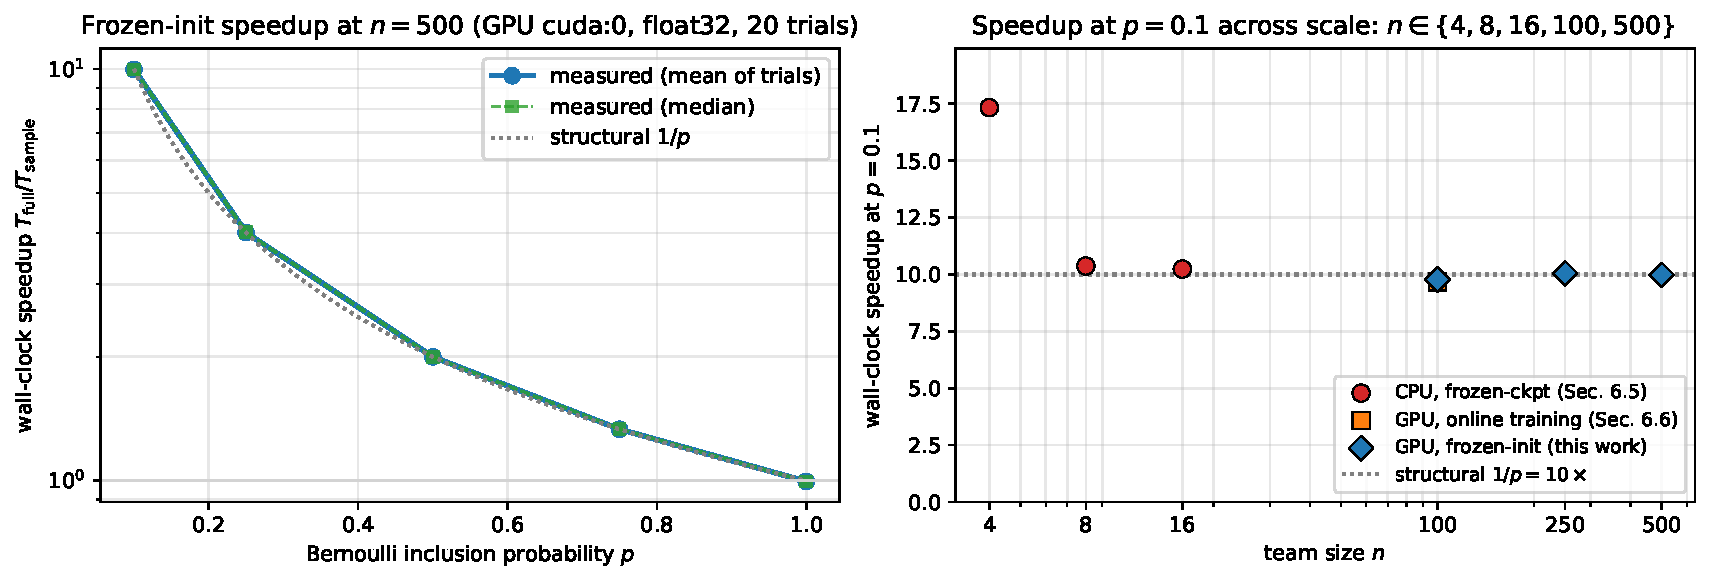
\includegraphics[width=0.85\linewidth]{figures/timing_n500.pdf}
\caption{Wall-clock scaling of $\widehat{\SND}(G_p)$ versus $\SND$
across $n\in\{4,\ldots,500\}$ and three hardware/call regimes.
\textbf{Left:} speedup $T_{\mathrm{full}} / T_{\mathrm{sampled}}$
versus Bernoulli $p$ at $n{=}500$ on a single RTX~4090 in fp32, 20
trials with \texttt{torch.cuda.synchronize}; dotted gray curve is
the structural $1/p$ prediction; markers show measured mean and
median (log-$y$).
\textbf{Right:} speedup at $p{=}0.1$ versus $n$, combining GPU
frozen-init (\emph{blue}, this section), CPU frozen-checkpoint
(\emph{red}, $n\in\{4,8,16\}$), and GPU online-training
(\emph{orange}, $n{=}100$; Section~\ref{sec:experiments:scaling}).
The dotted gray line at $10\times$ is the
$1/p=10\times$ prediction of
Proposition~\ref{prop:complexity}; speedups cluster around it across
the $125\times$ span of $n$ with no decay at scale.}
\label{fig:timing-n500}
\end{figure}

\subsection{Scaling to $n=100$ under real training dynamics}
\label{sec:experiments:scaling}

The frozen-init GPU sweep of Section~\ref{sec:experiments:timing}
isolates aggregation cost. To show that the same speedup and
concentration bounds hold \emph{under training}, we train $100$
independently parameterised Gaussian policies on VMAS Multi-Agent
Goal Navigation using the Section~\ref{sec:experiments:setup} IPPO
configuration, with scenario parameters auto-scaled for the larger
team ($\texttt{world\_spawning\_x}{=}\texttt{world\_spawning\_y}{=}4.0$,
$\texttt{agent\_radius}{=}0.03$, $\texttt{num\_envs}{=}32$). Every
$25$ PPO iterations we log $\SND(\mathbf{D})$ (all
$\binom{100}{2}{=}4{,}950$ pairs) and $\widehat{\SND}(G_{0.1})$
(one Bernoulli-$0.1$ subsample) together with per-call wall-clock,
timed with \texttt{cuda.synchronize} on both sides of every
\texttt{perf\_counter}.

Figure~\ref{fig:scaling-n100} reports the full trajectory. The
$\sim\!10\times$ speedup predicted by
Proposition~\ref{prop:complexity} is sustained throughout, staying in
$[9.0, 10.9]\times$ with no trend as policies diversify, and
$\widehat{\SND}(G_{0.1})$ tracks $\SND(\mathbf{D})$ essentially
indistinguishably (maximum gap $\sim 2\%$) at every one of $21$
logged iterations, extending the concentration guarantee of
Theorem~\ref{thm:concentration} from the frozen-checkpoint regime to
an active training run. The underlying $\SND$ trajectory itself
reflects realistic training dynamics (near-homogeneous init
$\to\,0.185$ peak at iter~$50$--$100$ $\to\,0.14$ steady state by
iter~$500$); the point is that Graph-SND tracks it correctly.

\begin{figure}[t]
\centering
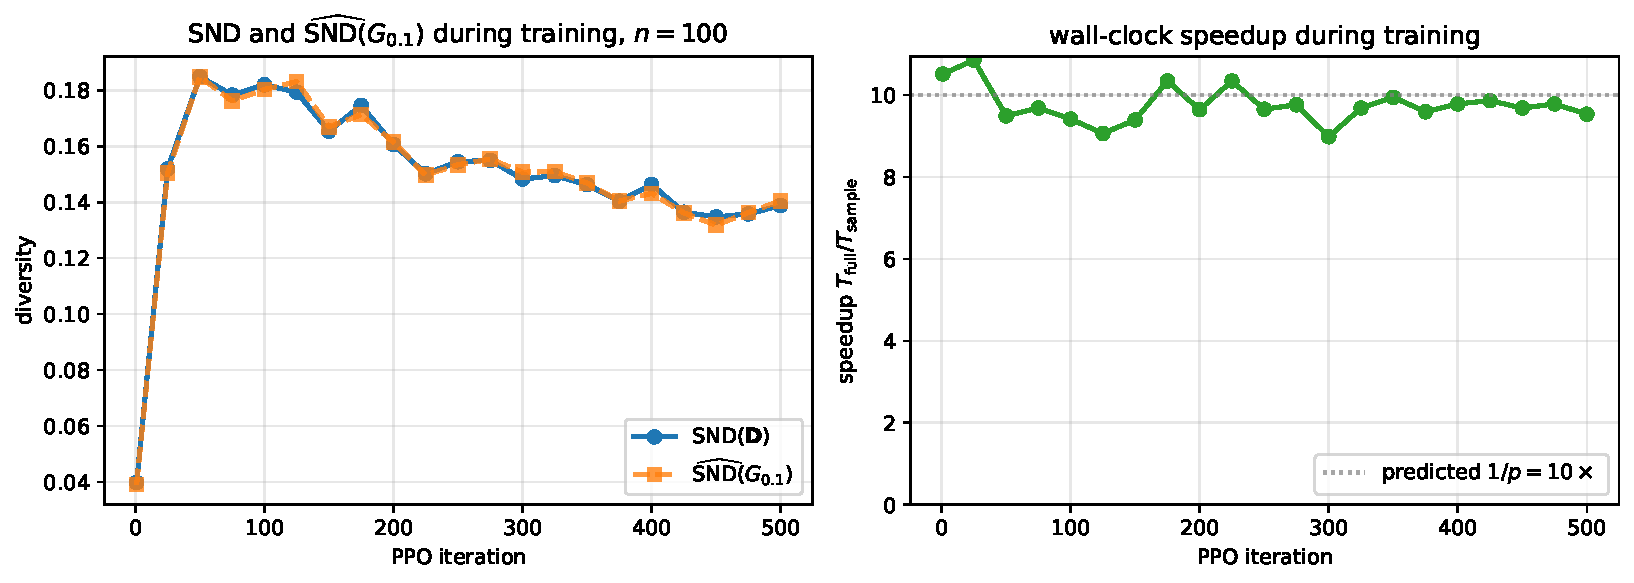
\includegraphics[width=0.85\linewidth]{figures/scaling_n100.pdf}
\caption{Graph-SND scaling on a $n=100$ PPO training run over 500
iterations. Left: $\SND(\mathbf{D})$ (full pairwise computation
over $\binom{100}{2} = 4{,}950$ pairs, blue) and
$\widehat{\SND}(G_{0.1})$ (Horvitz--Thompson estimator on a
Bernoulli-$0.1$ subsample, orange) evaluated on the current rollout
batch every 25 iterations. The two curves overlap visually
throughout, validating Theorem~\ref{thm:concentration} under
non-stationary training dynamics. Right: wall-clock speedup
$T_{\mathrm{full}}/T_{\mathrm{sample}}$ per measurement, stable
around the predicted $1/p = 10\times$ ratio.}
\label{fig:scaling-n100}
\end{figure}

\paragraph{Interpretation.} At $n{=}100$ full $\SND$ costs
$\approx\!1.2\,$s of aggregation per measurement and the sampled
estimator reduces this to $\approx\!0.12\,$s while preserving the
measurement to within noise. For any downstream use that queries
diversity inside a training loop---for example, DiCo
\citep{bettini2024dico}---this is the difference between a
negligible overhead and a measurable fraction of update time.

\subsection{Closed-loop diversity control on VMAS Dispersion}
\label{sec:experiments:dico-dispersion}

To demonstrate downstream utility beyond frozen-policy measurement,
we integrate Graph-SND into the DiCo heterogeneity controller of
\citet{bettini2024dico} on VMAS Dispersion \citep{bettini2022vmas}
with $n{=}10$ agents, ten food targets, shared team reward, and
Independent PPO with the HetControl heterogeneous MLP
\citep{bettini2024dico}. DiCo regularises training toward a target
diversity $\SND_{\mathrm{des}}$ using the full $O(n^2)$ aggregator;
we replace that aggregator with Graph-SND on either a dynamic
per-environment $k$-nearest-neighbour graph ($k{=}3$ in observation
space, $128$-env subsample) or a Bernoulli-$0.1$ random subgraph. We
compare four configurations at matched training budget ($167$
iterations, ${\approx}10^7$ frames) across three seeds: diversity
control disabled (\texttt{desired\_snd}${=}{-}1$), DiCo with full
pairwise $\SND$ on $K_n$, DiCo with $k$-NN Graph-SND, and DiCo with
Bernoulli-$0.1$ Graph-SND; all controlled runs use
$\SND_{\mathrm{des}}{=}0.1$.

Figure~\ref{fig:dico-dispersion-knn} summarises the four runs along
three axes (reward, applied-$\SND$ tracking, per-call metric cost).
Terminal mean reward (last $10$ iterations, three seeds) is
$0.070\pm0.001$ for Bernoulli-$0.1$, $0.069\pm0.003$ for $k$-NN,
$0.064\pm0.001$ for full $\SND$, and $0.056\pm0.003$ for the
diversity-off baseline: both sparse variants match full $\SND$
within seed variance and all three controlled runs outperform
unconstrained IPPO. All controlled variants hold the \emph{applied}
$\SND$ (post-scaling, \citep{bettini2024dico}) at
$0.1010\pm0.0004$ (full), $0.1009\pm0.0003$ ($k$-NN), and
$0.1007\pm0.0005$ (Bernoulli-$0.1$), indistinguishable from the
$\SND_{\mathrm{des}}{=}0.1$ set point to within $10^{-3}$. Median
per-call metric cost is $0.53\,\text{ms}$ (full), $0.24\,\text{ms}$
($k$-NN), $0.15\,\text{ms}$ (Bernoulli-$0.1$)---median speedups of
$2.16\times$ ($k$-NN) and $3.63\times$ (Bernoulli-$0.1$), matching
the pair-count ratios $\binom{n}{2}:nk/2:0.1\binom{n}{2}$ implied by
Proposition~\ref{prop:complexity} at $n{=}10$. Sparse Graph-SND is
therefore jointly (i) a faithful drop-in at the DiCo metric API,
(ii) at no cost to downstream reward, and (iii) at reduced per-call
metric cost even at modest $n$. Fixed-$G$ ($k$-NN) and random-$G$
(Bernoulli-$0.1$) provide complementary operating points in the
same controller ($k$-NN preserves structured locality;
Bernoulli-$0.1$ minimises metric cost). Absolute per-call times here
are GPU-measured inside the DiCo training loop at the minibatched
rollout shape and so have a different magnitude than the
frozen-checkpoint CPU timings of Section~\ref{sec:experiments:timing}
and the in-training GPU timings of
Section~\ref{sec:experiments:scaling}; the invariant across all three
regimes is the $\binom{n}{2}/|E|$ ratio of
Proposition~\ref{prop:complexity}.

\begin{figure}[t]
\centering
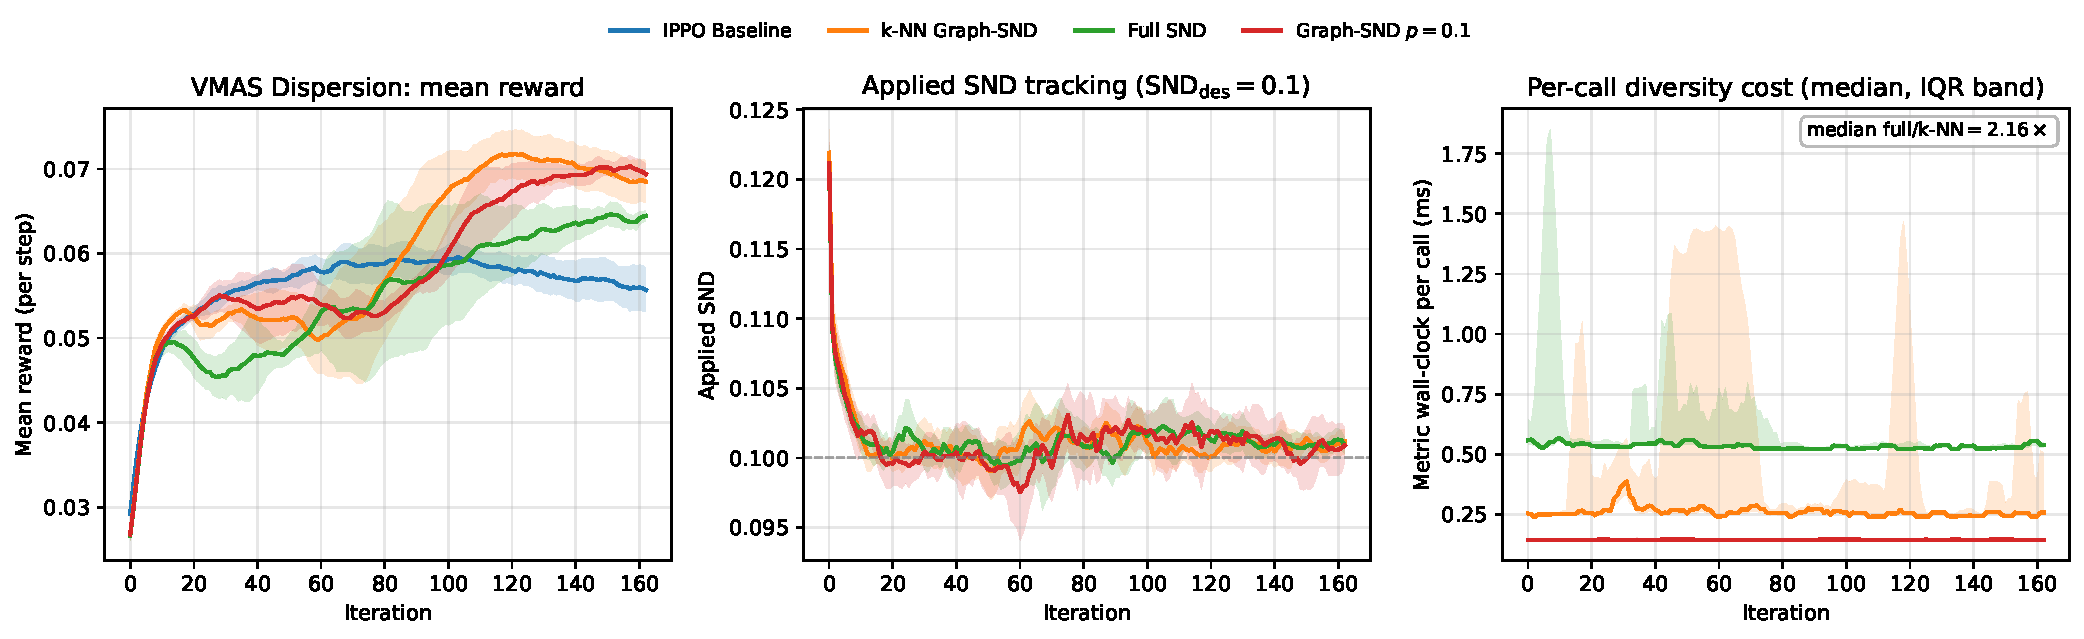
\includegraphics[width=0.88\linewidth]{figures/neurips_knn_plot.pdf}
\caption{DiCo with Graph-SND on VMAS Dispersion with shared reward
($n{=}10$, ten foods, $\SND_{\mathrm{des}}{=}0.1$, three seeds).
\textbf{Blue:} IPPO baseline, diversity control disabled
(\texttt{desired\_snd}${=}{-}1$). \textbf{Green:} DiCo with full
pairwise $\SND$ on $K_n$. \textbf{Orange:} DiCo with $k$-NN Graph-SND
($k{=}3$, $128$ environments subsampled for the $k$-NN construction).
\textbf{Red:} DiCo with Bernoulli-$0.1$ Graph-SND
(\texttt{diversity\_estimator=graph\_p01}).
Lines are mean over seeds; bands are mean~$\pm$~std for reward
(Panel~1) and applied SND (Panel~2), and median with IQR for per-call
metric cost (Panel~3)---timing data is right-skewed, so median/IQR is
robust to sparse CUDA-sync tail events. Panel~1: all three DiCo
variants outperform the diversity-off baseline; both sparse Graph-SND
variants are within seed variance of full $\SND$. Panel~2: all
controlled runs track $\SND_{\mathrm{des}}{=}0.1$ to within $10^{-3}$.
Panel~3: median per-call cost is lowest for Bernoulli-$0.1$, then
$k$-NN, then full $\SND$, matching the expected pair-count ordering;
the annotation reports both median speedups over full $\SND$. Both
sparse variants exhibit sparse IQR widening from CUDA-sync tail
events: the $k$-NN band reflects occasional graph-construction
spikes on the $128$-env subsample, while the Bernoulli-$0.1$ band
reflects per-call sampling-mask variance. In both cases the
worst-case per-call cost remains bounded by the full-$\SND$ cost
plus a constant overhead (graph construction for $k$-NN,
mask+$1/p$ reweighting for Bernoulli-$0.1$).}
\label{fig:dico-dispersion-knn}
\end{figure}

% ============================================================
\section{Discussion}
\label{sec:discussion}

Graph-SND replaces the aggregation step of $\SND$ with a
graph-parameterised construction that recovers $\SND$ exactly on
$K_n$ and scales linearly in $|E|$. The two interpretations of
$\SNDG$ correspond to two commitments: a fixed $G$ is a
\emph{modeling} commitment (only certain agent pairs matter, per
Remark~\ref{rem:semantics}), while a random $G$ with
Horvitz--Thompson weights is an \emph{estimation} commitment
(full $\SND$ is the target, sparsity is computational); their
guarantees are complementary (exact recovery/invariance versus
unbiasedness/concentration and the fixed-$G$ distortion bound of
Theorem~\ref{thm:distortion}, which ties MARL diversity aggregation to
classical edge-congestion / multicommodity-flow results on
graphs~\citep{chung1987forwarding,heydemann1989forwarding,leighton1999multicommodity}).
The most immediate downstream application is DiCo
\citep{bettini2024dico}: $\SNDG$ drops in as the control target, with
$G$ selecting between local diversity control and a compute-subsampled
variant, as validated on VMAS Dispersion.

\paragraph{Limitations.}
We flag five scope limits.
\emph{(1) Scale and timing regime:} property-level verifications
(Appendix~\ref{app:verify}) reach only $n{=}16$; online PPO reaches
$n{=}100$ and frozen-init GPU timing reaches $n{=}500$ across four
hardware/call regimes, but we rely on the $\binom{n}{2}/|E|$
\emph{ratio} rather than absolute times, and training $n\gg 100$
IPPO agents is out of scope.
\emph{(2) Scenario and DiCo-configuration coverage:} non-DiCo
experiments use only Multi-Agent Goal Navigation
\citep{bettini2025snd}; the DiCo integration uses Dispersion at a
single $\SND_{\mathrm{des}}{=}0.1$ over three seeds.
\emph{(3) Fixed-$G$ ablation outside DiCo:} the only structured fixed
$G$ we exercise is the $k$-NN graph inside DiCo;
Theorem~\ref{thm:distortion} bounds worst-case distortion for
arbitrary fixed $G$, but distribution-dependent sharpenings and an
expander-design ablation are untested.
\emph{(4) Closed-form Wasserstein assumption:} every computational
result uses the Gaussian closed form of \citet{bettini2025snd};
the theorems hold for any bounded $d(i,j)\in[0,D_{\max}]$, but we
do not verify on a non-Gaussian family.
\emph{(5) IPPO-only algorithm scope:} every RL result uses
Independent PPO; extending to centralised-critic and other
policy-gradient algorithms covered by DiCo is a straightforward but
untested extension.

\paragraph{Future work.}
Beyond closing these limits, four directions are natural:
(i) \emph{learned or task-adaptive $G$}; (ii) \emph{non-Gaussian
policies} by substituting a closed-form or approximate $d$;
(iii) \emph{distribution-dependent tightenings} of
Theorem~\ref{thm:distortion} and an empirical expander-graph $G$
study; and (iv) a broader DiCo$+\SNDG$ study, over larger $n$, tasks,
set-points, and the interaction of sampling noise in
$\widehat{\SND}(G_p)$ with DiCo's set-point regulation.
\section{Conclusion}
\label{sec:conclusion}

We introduced Graph-SND, replacing SND's $\binom{n}{2}$-pair average
with a normalised weighted mean over the edges of a user-specified
graph $G$: a localised diversity measure for fixed $G$, and an
unbiased Horvitz--Thompson sampling estimator of $\SND$ for random
$G$. Seven formal results and experiments across
$n\in\{4,8,16,100,250,500\}$ on VMAS Goal Navigation and a DiCo closed
loop on Dispersion confirm that $\SNDG$ is a drop-in replacement for
$\SND$: recovery is numerically exact, concentration is respected on
every cell, wall-clock cost tracks $\binom{n}{2}/|E|$ across a
$125\times$ span of $n$, and both $k$-NN and Bernoulli-$0.1$
substitutions inside DiCo match the full-$\SND$ set point to within
$10^{-3}$ and full-$\SND$ reward within seed variance. The choice of
$G$ selects whether the signal measures local diversity or
approximates global diversity at reduced cost.
\codelocation

% ============================================================
% References are unlimited and do NOT count toward the 9-page main
% content budget. They appear here right after the conclusion.
\bibliographystyle{plainnat}
\bibliography{references}

% ============================================================
% Acknowledgments and Disclosure of Funding
% ------------------------------------------------------------
% The NeurIPS style file automatically hides this block in
% anonymous-submission mode (\usepackage{neurips_2026} with the default
% "main" option) and shows it in preprint / final mode. Any
% funding-source or named-person acknowledgements must live here and
% only here; never include them inside the main text or abstract.
\begin{ack}
The author thanks Matteo Bettini and the ProrokLab for the System
Neural Diversity implementation and the VMAS \& DiCo open-source
releases on which this work builds.
\end{ack}

% ============================================================
% NeurIPS Paper Checklist (mandatory; does not count toward page limit).
\section*{NeurIPS Paper Checklist}

\begin{enumerate}

\item {\bf Claims}
    \item[] Question: Do the main claims made in the abstract and introduction accurately reflect the paper's contributions and scope?
    \item[] Answer: \answerYes{}
    \item[] Justification: The abstract and Section~\ref{sec:intro}
    state exactly the four claims validated by the experiments
    (recovery, unbiasedness, concentration, and wall-clock speedup),
    with the downstream DiCo integration flagged separately, and each
    claim is numbered and cross-referenced. The scope restrictions
    (IPPO only, VMAS Multi-Agent Goal Navigation and Dispersion, fixed
    Gaussian policies; the main DiCo experiment is at a single set
    point $\SND_{\mathrm{des}}{=}0.1$, with a three-seed, three-set-point
    sweep at $n{=}50$ in Appendix~\ref{app:dico-n50-sweep}) are stated in
    Section~\ref{sec:discussion} (Limitations) and do not contradict
    any claim in the abstract or introduction.

\item {\bf Limitations}
    \item[] Question: Does the paper discuss the limitations of the work performed by the authors?
    \item[] Answer: \answerYes{}
    \item[] Justification: Section~\ref{sec:discussion} contains a
    dedicated ``Limitations'' paragraph itemising five scope limits
    (scale/timing regime coverage, scenario and DiCo-configuration
    coverage, fixed-$G$ ablation, closed-form Wasserstein assumption,
    IPPO-only scope).

\item {\bf Theory assumptions and proofs}
    \item[] Question: For each theoretical result, does the paper provide the full set of assumptions and a complete (and correct) proof?
    \item[] Answer: \answerYes{}
    \item[] Justification: All seven formal results
    (Propositions~\ref{prop:recovery}--\ref{prop:unbiased},
    Theorem~\ref{thm:concentration}, and Theorem~\ref{thm:distortion})
    are proved in full in Appendix~\ref{app:proofs}.
    Propositions~\ref{prop:recovery}--\ref{prop:unbiased} and
    Theorem~\ref{thm:concentration} are stated with their assumptions in
    Sections~\ref{sec:method}--\ref{sec:theory}; Theorem~\ref{thm:distortion}
    is stated in Appendix~\ref{app:proofs} with a compact summary in
    Section~\ref{sec:theory}. Assumptions (e.g.,
    non-negative edge weights with $W(G)>0$, bounded distances
    $d(i,j)\in[0,D_{\max}]$, independent Bernoulli inclusion under
    Horvitz--Thompson weights) are stated inside the corresponding
    theorem statements and reused verbatim in the proofs.

\item {\bf Experimental result reproducibility}
    \item[] Question: Does the paper fully disclose all the information needed to reproduce the main experimental results of the paper?
    \item[] Answer: \answerYes{}
    \item[] Justification: Section~\ref{sec:experiments:setup}
    specifies the VMAS environment, team sizes, policy architecture,
    training algorithm (IPPO), checkpoints (iter~0, iter~100), rollout
    set size, and metric implementation. Appendix~\ref{app:hyperparams}
    lists every PPO hyperparameter and the $n{=}100$ scaling overrides.
    The frozen-init GPU timing sweep and the DiCo integration
    (Sections~\ref{sec:experiments:timing},
    \ref{sec:experiments:dico-dispersion}) specify batch
    shape, timing regime (\texttt{torch.cuda.synchronize} on both
    sides of every \texttt{perf\_counter}), number of trials, number
    of seeds, and configuration of the $k$-NN graph and the Bernoulli
    random graph. The $n{=}50$ set-point sweep
    (Appendix~\ref{app:dico-n50-sweep}) reuses these hyperparameters
    except for the reduced per-iteration rollout
    (\texttt{on\_policy\_n\_envs\_per\_worker}${=}120$,
    \texttt{on\_policy\_collected\_frames\_per\_batch}${=}12{,}000$)
    and is driven by
    \texttt{ControllingBehavioralDiversity-fork/scripts/launch\_n50\_bern\_setpoint\_sweep.sh}.
    Everything needed to reconstruct the code paths is
    in \texttt{graphsnd/metrics.py}, \texttt{graphs.py},
    \texttt{training/train\_navigation\_batched.py}, and
    \texttt{experiments/exp2\_timing\_scaling.py} in the companion
    repository.

\item {\bf Open access to data and code}
    \item[] Question: Does the paper provide open access to the data and code, with sufficient instructions to faithfully reproduce the main experimental results, as described in supplemental material?
    \item[] Answer: \answerYes{}
    \item[] Justification: All code is released at the repository
    cited in the Conclusion, with a top-level \texttt{README.md}
    that specifies installation, training, experiment reproduction
    commands, and seed-42 expected values for each of the four
    validated claims. Raw CSVs, summary JSONs, and figure PDFs for
    every experiment in the paper are checked into the repository
    under \texttt{results/}. A preflight script
    (\texttt{scripts/preflight.sh}) runs the test suite and a
    smoke-training pass on each visible CUDA device to catch
    environment problems before overnight runs. For the anonymous
    submission the repository URL is anonymised in the main text;
    the supplementary material contains an anonymised snapshot.

\item {\bf Experimental setting/details}
    \item[] Question: Does the paper specify all the training and test details necessary to understand the results?
    \item[] Answer: \answerYes{}
    \item[] Justification: Training details (optimiser, learning
    rate, clip parameter, GAE $\lambda$, discount $\gamma$, rollout
    shape, mini-batch size, PPO epochs, hidden-layer width, activation)
    are listed in Appendix~\ref{app:hyperparams}. The DiCo integration
    of Section~\ref{sec:experiments:dico-dispersion} additionally
    specifies the HetControl architecture, $\SND_{\mathrm{des}}{=}0.1$
    set point, $167$-iteration budget, three seeds, $k{=}3$ for the
    $k$-NN graph, Bernoulli inclusion probability $p{=}0.1$, and the
    $128$-env subsample used for the $k$-NN construction. The
    supplementary $n{=}50$ set-point sweep
    (Appendix~\ref{app:dico-n50-sweep}) uses the same $167$-iteration
    budget, three seeds per cell, $p{=}0.1$, and three set points
    $\SND_{\mathrm{des}}\in\{0.12,0.14,0.15\}$.

\item {\bf Experiment statistical significance}
    \item[] Question: Does the paper report error bars suitably and correctly defined or other appropriate information about the statistical significance of the experiments?
    \item[] Answer: \answerYes{}
    \item[] Justification: The unbiasedness diagnostic
    (Section~\ref{sec:experiments:verify}, Appendix~\ref{app:verify})
    reports $95\%$ confidence intervals from $2{,}000$ Bernoulli draws
    per $p$ and the standardised deviation
    $|\mathrm{bias}|/\mathrm{SE}$ as a sharper test. The concentration
    diagnostic reports the empirical violation rate at $\delta{=}0.1$
    over $2{,}000$ draws per cell and the $95$th-percentile deviation.
    The timing experiments
    (Section~\ref{sec:experiments:timing},
    \ref{sec:experiments:scaling}) report mean, median, and standard
    deviation over $20$ timing trials per cell after $3$ warm-ups.
    The DiCo experiment (Section~\ref{sec:experiments:dico-dispersion})
    reports mean $\pm$ standard deviation over three seeds for reward
    and applied SND, and median with IQR for per-call metric cost.
    The $n{=}50$ set-point sweep (Appendix~\ref{app:dico-n50-sweep},
    Table~\ref{tab:dico-n50-sweep}) reports late-window (last
    $50$ iterations) means $\pm$ cross-seed standard error over three
    seeds per set point and the relative tracking error
    $\overline{|\mathrm{applied}\;\SND-\SND_{\mathrm{des}}|}/
    \SND_{\mathrm{des}}$.

\item {\bf Experiments compute resources}
    \item[] Question: For each experiment, does the paper provide sufficient information on the computer resources needed to reproduce the experiments?
    \item[] Answer: \answerYes{}
    \item[] Justification: The $n{\in}\{4,8,16\}$ frozen-checkpoint
    verifications (Section~\ref{sec:experiments:verify},
    Appendix~\ref{app:verify}) run on a single CPU core with the
    reported $20$ trials per cell in minutes. The $n{=}100$ overnight
    PPO run (Section~\ref{sec:experiments:scaling}) fits on one
    RTX~4090, as does the frozen-init $n\in\{100,250,500\}$ GPU timing
    sweep (Section~\ref{sec:experiments:timing}). The DiCo
    closed-loop experiment
    (Section~\ref{sec:experiments:dico-dispersion}) also
    runs on one RTX~4090 at the reported $167$-iteration budget.
    The supplementary $n{=}50$ set-point sweep
    (Appendix~\ref{app:dico-n50-sweep}, nine cells of three seeds
    $\times$ three set points) runs sequentially on one RTX~4090 at
    ${\approx}2$ GPU-hours per cell (${\approx}18$ GPU-hours total).
    Total compute for the experiments reported in this paper is
    under $48$ GPU-hours on one RTX~4090 plus a few CPU-hours for
    the $n{\in}\{4,8,16\}$ benchmarks.

\item {\bf Code of ethics}
    \item[] Question: Does the research conducted in the paper conform, in every respect, with the NeurIPS Code of Ethics?
    \item[] Answer: \answerYes{}
    \item[] Justification: The work is theoretical and empirical
    research on a metric for behavioural diversity in cooperative
    MARL. It does not involve human subjects, sensitive data, or
    release of models with plausible misuse potential. No deviations
    from the NeurIPS Code of Ethics are required.

\item {\bf Broader impacts}
    \item[] Question: Does the paper discuss both potential positive societal impacts and negative societal impacts of the work performed?
    \item[] Answer: \answerNA{}
    \item[] Justification: Graph-SND is a methodological metric
    contribution that reduces the wall-clock cost of measuring
    behavioural diversity in cooperative MARL. It enables neither
    new capabilities nor new deployments; it only makes an existing
    measurement cheaper. We therefore do not identify a direct path
    to positive or negative societal impact.

\item {\bf Safeguards}
    \item[] Question: Does the paper describe safeguards that have been put in place for responsible release of data or models that have a high risk for misuse?
    \item[] Answer: \answerNA{}
    \item[] Justification: No data or models with misuse potential
    are released; the released artefacts are experimental code,
    reproducible CSV/JSON result files, and paper figures.

\item {\bf Licenses for existing assets}
    \item[] Question: Are the creators or original owners of assets used in the paper properly credited and are the license and terms of use explicitly mentioned and properly respected?
    \item[] Answer: \answerYes{}
    \item[] Justification: VMAS \citep{bettini2022vmas} and DiCo
    \citep{bettini2024dico} are credited in the main text and
    released under their original open-source licenses. The vendored
    fork of the DiCo codebase in
    \texttt{ControllingBehavioralDiversity-fork/} retains the
    upstream license, adds a \texttt{GRAPH\_SND\_CHANGES.md} file
    documenting the modifications, and includes the preferred
    citation in \texttt{CITATION.cff}. The original SND paper
    \citep{bettini2025snd} is cited throughout.

\item {\bf New assets}
    \item[] Question: Are new assets introduced in the paper well documented and is the documentation provided alongside the assets?
    \item[] Answer: \answerYes{}
    \item[] Justification: The new assets are the \texttt{graphsnd}
    Python package, the two training scripts, the experiment
    scripts, and the released figure and CSV outputs. The top-level
    \texttt{README.md} documents installation, the four entry-point
    experiments, the overnight training launcher, and the repository
    layout, and cross-references the specific paper sections that
    each asset reproduces.

\item {\bf Crowdsourcing and research with human subjects}
    \item[] Question: For crowdsourcing experiments and research with human subjects, does the paper include the full text of instructions given to participants and screenshots, if applicable, as well as details about compensation?
    \item[] Answer: \answerNA{}
    \item[] Justification: No crowdsourcing or human-subjects
    research is involved.

\item {\bf Institutional review board (IRB) approvals or equivalent for research with human subjects}
    \item[] Question: Does the paper describe potential risks incurred by study participants, whether such risks were disclosed to the subjects, and whether IRB approvals (or equivalent) were obtained?
    \item[] Answer: \answerNA{}
    \item[] Justification: No human-subjects research is involved.

\item {\bf Declaration of LLM usage}
    \item[] Question: Does the paper describe the usage of LLMs if it is an important, original, or non-standard component of the core methods in this research?
    \item[] Answer: \answerNA{}
    \item[] Justification: No LLM is part of the methods, theory,
    or experimental pipeline of this paper. LLMs were used only as
    writing / editing assistance and do not affect the core
    methodology, scientific rigour, or originality of the research.

\end{enumerate}


% ============================================================
% Appendix: proofs, hyperparameters, and empirical verification.
\appendix
\section{Proofs}
\label{app:proofs}

We use the conventions of Section~\ref{sec:background}: $\Agents$ is the
agent set with $|\Agents| = n$; $\Pairs = \binom{\Agents}{2}$ is the set
of unordered agent pairs, with $|\Pairs| = \binom{n}{2}$; $d(i,j) \geq 0$
is the Monte Carlo behavioral distance~\eqref{eq:dij}, treated as a
deterministic scalar given the rollout set $\Rollouts$; and $G = (\Agents,
E, w)$ has non-negative edge weights $w_{ij}$ with total weight
$W(G) = \sum_{\{i,j\} \in E} w_{ij} > 0$.

\subsection*{Proof of Proposition~\ref{prop:recovery} (Recovery)}

If $G = K_n$ with $w_{ij} = 1$ for all $\{i,j\} \in \Pairs$, then
$E = \Pairs$ and $W(G) = |\Pairs| = \binom{n}{2}$. Substituting
into~\eqref{eq:graph-snd},
\[
\SNDG(\mathbf{D}, K_n)
\;=\; \frac{1}{\binom{n}{2}} \sum_{\{i,j\} \in \Pairs} 1 \cdot d(i,j)
\;=\; \binom{n}{2}^{-1} \sum_{i < j} d(i,j)
\;=\; \SND(\mathbf{D}). \qed
\]

\subsection*{Proof of Proposition~\ref{prop:nonneg} (Non-negativity)}

Each term $w_{ij} d(i,j)$ in~\eqref{eq:graph-snd} is a product of
non-negative factors, so the numerator $\sum_{E} w_{ij} d(i,j) \geq 0$.
Since $W(G) > 0$ by assumption, $\SNDG(\mathbf{D}, G) \geq 0$.

For the equality condition, $\SNDG = 0$ iff
$\sum_{\{i,j\} \in E} w_{ij} d(i,j) = 0$. A sum of non-negative terms is
zero iff each term is zero, so the equality holds iff $w_{ij} d(i,j) = 0$
for every $\{i,j\} \in E$. Equivalently, $d(i,j) = 0$ for every edge
$\{i,j\} \in E$ with $w_{ij} > 0$. \qed

\subsection*{Proof of Proposition~\ref{prop:perm} (Automorphism invariance)}

Let $\sigma : \Agents \to \Agents$ be an automorphism of $(G, w)$, meaning
$\sigma$ is a bijection satisfying $\{i,j\} \in E \iff \{\sigma(i),
\sigma(j)\} \in E$ and $w_{ij} = w_{\sigma(i)\sigma(j)}$ for all
$\{i,j\} \in E$. Then
\begin{align*}
\SNDG(\sigma \cdot \mathbf{D}, G)
&\;=\; \frac{1}{W(G)} \sum_{\{i,j\} \in E} w_{ij}\, d(\sigma(i), \sigma(j)).
\end{align*}
Reindex the sum by $\{i', j'\} = \{\sigma(i), \sigma(j)\}$. Because
$\sigma$ is an automorphism, the map $\{i,j\} \mapsto \{\sigma(i),
\sigma(j)\}$ is a bijection $E \to E$, and $w_{ij} =
w_{\sigma(i)\sigma(j)} = w_{i'j'}$. Hence
\[
\SNDG(\sigma \cdot \mathbf{D}, G)
\;=\; \frac{1}{W(G)} \sum_{\{i',j'\} \in E} w_{i'j'}\, d(i', j')
\;=\; \SNDG(\mathbf{D}, G). \qed
\]

\subsection*{Proof of Proposition~\ref{prop:complexity} (Complexity)}

Evaluating~\eqref{eq:graph-snd} on a precomputed graph $G$ reduces to
computing $d(i,j)$ for each $\{i,j\} \in E$ and forming a weighted sum. The
sum costs $O(|E|)$ floating-point operations, dominated by the $|E|$
pairwise-distance computations. $\SND$ in~\eqref{eq:snd} instead requires
$|\Pairs| = \binom{n}{2}$ such computations. Since each pairwise-distance
computation has the same cost in both cases, the speedup factor in the
number of pairwise-distance evaluations is $\binom{n}{2}/|E|$. For $k$-NN
graphs $|E| = O(nk)$, giving a factor of $\Theta(n/k)$. This statement
does not include the cost of constructing $G$. \qed

\subsection*{Proof of Proposition~\ref{prop:unbiased} (Unbiasedness)}

For each $\{i,j\} \in \Pairs$, let $Z_{ij} = \ind[\{i,j\} \in E(G_p)]$.
By construction, $\{Z_{ij}\}_{\{i,j\} \in \Pairs}$ are independent
Bernoulli$(p)$ random variables. With $w_{ij} = 1/p$ on edges of $G_p$,
\[
\widehat{\SND}(G_p)
\;=\; |\Pairs|^{-1} \sum_{\{i,j\} \in E(G_p)} w_{ij}\, d(i,j)
\;=\; |\Pairs|^{-1} \sum_{\{i,j\} \in \Pairs} Z_{ij} \cdot \tfrac{1}{p}
\cdot d(i,j).
\]
Taking expectation and using $\E[Z_{ij}] = p$,
\[
\E_{G_p}\!\left[\widehat{\SND}(G_p)\right]
\;=\; |\Pairs|^{-1} \sum_{\{i,j\} \in \Pairs}
p \cdot \tfrac{1}{p} \cdot d(i,j)
\;=\; |\Pairs|^{-1} \sum_{\{i,j\} \in \Pairs} d(i,j)
\;=\; \SND(\mathbf{D}). \qed
\]

\subsection*{Proof of Theorem~\ref{thm:concentration} (Concentration)}

We first establish that, conditional on $|E(G_p)| = m$, $E(G_p)$ is a
uniform random subset of $\Pairs$ of size $m$.

\begin{lemma}
\label{lem:conditional-uniform}
Let $\{Z_\alpha\}_{\alpha \in \Pairs}$ be i.i.d.\ Bernoulli$(p)$ with
$p \in (0,1)$, and let $E = \{\alpha : Z_\alpha = 1\}$. Conditional on
$|E| = m$ with $0 \leq m \leq |\Pairs|$, the set $E$ is uniformly
distributed over subsets of $\Pairs$ of size $m$.
\end{lemma}
\begin{proof}
For any fixed $T \subseteq \Pairs$ with $|T| = m$,
\[
\Prob(E = T \mid |E| = m)
\;=\; \frac{\Prob(E = T)}{\Prob(|E| = m)}
\;=\; \frac{p^m (1-p)^{|\Pairs|-m}}
          {\binom{|\Pairs|}{m} p^m (1-p)^{|\Pairs|-m}}
\;=\; \binom{|\Pairs|}{m}^{-1},
\]
which does not depend on $T$.
\end{proof}

Now fix $m \geq 1$ and condition on $|E(G_p)| = m$. By
Lemma~\ref{lem:conditional-uniform}, $E(G_p)$ is a uniform random sample
of size $m$ without replacement from the finite population
\[
\Pi \;:=\; \bigl\{ d(i,j) : \{i,j\} \in \Pairs \bigr\},
\]
where $|\Pi| = |\Pairs|$ and each $d(i,j) \in [0, D_{\max}]$. The
population mean is
\[
\mu \;:=\; |\Pairs|^{-1} \sum_{\{i,j\} \in \Pairs} d(i,j) \;=\; \SND(\mathbf{D}),
\]
and the sample mean is precisely
\[
\SNDG^{\mathrm{u}}(\mathbf{D}, G_p) \;=\; m^{-1} \sum_{\{i,j\} \in E(G_p)} d(i,j).
\]

\citet[Section 6, Theorem 4]{hoeffding1963probability} establishes that
the two-sided Hoeffding inequality applies to sampling without
replacement from a bounded finite population: for any $t > 0$,
\begin{equation}
\label{eq:hoeff-wor}
\Prob\bigl(\abs{\SNDG^{\mathrm{u}} - \SND} \geq t \;\bigm|\; |E(G_p)| = m\bigr)
\;\leq\; 2\exp\!\left(- \frac{2 m t^2}{D_{\max}^2}\right).
\end{equation}
Setting the right-hand side equal to $\delta$ and solving for $t$ gives
\[
t \;=\; D_{\max}\sqrt{\frac{\log(2/\delta)}{2m}}.
\]
Thus with probability at least $1 - \delta$ conditional on $|E(G_p)| = m$,
\[
\abs{\SNDG^{\mathrm{u}}(\mathbf{D}, G_p) - \SND(\mathbf{D})}
\;\leq\; D_{\max}\sqrt{\frac{\log(2/\delta)}{2m}}. \qed
\]

\subsection*{Deterministic fixed-$G$ distortion}
\label{app:distortion}

For a connected unit-weight graph $G=(\Agents,E)$, a \emph{path system}
is an assignment of a simple $i$-$j$ path $\mathcal{R}_{ij}\subseteq E$
to every pair $\{i,j\}\in\Pairs$, with
$\mathcal{R}_{ij}=\{\{i,j\}\}$ whenever $\{i,j\}\in E$. The
\emph{congestion} of a path system $\mathcal{R}$ at an edge
$\{a,b\}\in E$ is
$c_{\mathcal{R}}(a,b):=\abs{\{\{i,j\}\in\Pairs :
\{a,b\}\in\mathcal{R}_{ij}\}}$, and the \emph{edge forwarding index} of
$G$ is
$\pi(G):=\min_{\mathcal{R}} \max_{\{a,b\}\in E} c_{\mathcal{R}}(a,b)$
\citep{chung1987forwarding,heydemann1989forwarding}. The index depends
on $G$ alone, satisfies $\pi(K_n)=1$, admits closed forms for many
graph families (hypercubes, tori, Cayley graphs), and is
$\mathcal{O}(n\log n / d)$ for $d$-regular graphs with bounded spectral
gap~\citep{leighton1999multicommodity}.

\begin{theorem}[Deterministic fixed-$G$ distortion]
\label{thm:distortion}
Let $G=(\Agents, E)$ be a connected graph with unit edge weights, and
suppose $d:\Pairs\to\R_{\geq 0}$ satisfies the triangle inequality
$d(i,j)\leq d(i,k)+d(k,j)$ for all $i,j,k\in\Agents$ (automatic for
the Monte Carlo distance~\eqref{eq:dij}, since $\Wass$ is a metric).
Writing $\SNDG^{\mathrm{u}}(\mathbf{D},G):=|E|^{-1}\sum_{\{i,j\}\in E}
d(i,j)$ for the unit-weight variant of $\SNDG$,
\begin{equation}
\label{eq:distortion}
\frac{|E|}{|\Pairs|}\,\SNDG^{\mathrm{u}}(\mathbf{D}, G)
\;\leq\; \SND(\mathbf{D})
\;\leq\; \frac{|E|\,\pi(G)}{|\Pairs|}\,\SNDG^{\mathrm{u}}(\mathbf{D}, G),
\end{equation}
so $|E|/|\Pairs|\leq\SND(\mathbf{D})/\SNDG^{\mathrm{u}}(\mathbf{D},G)\leq|E|\pi(G)/|\Pairs|$ whenever $\SNDG^{\mathrm{u}}>0$; both ratios are
$1$ on $K_n$, recovering Proposition~\ref{prop:recovery}.
\end{theorem}

\begin{corollary}[Expander sparsification]
\label{cor:expander-distortion}
If $G$ is a $d$-regular graph on $n$ vertices with bounded spectral
gap (e.g.\ a spectral expander or a random $d$-regular graph), then
Theorem~\ref{thm:distortion} and $\pi(G)=\mathcal{O}(n\log n/d)$ give
$|E|/|\Pairs|=d/(n-1)$ and $|E|\pi(G)/|\Pairs|=\mathcal{O}(\log n)$.
Choosing $d=\Theta(\log n)$ yields $|E|=\Theta(n\log n)$ pairwise
distance evaluations with worst-case relative distortion
$\mathcal{O}(\log n)$, a $\Theta(n/\log n)$-factor reduction against
full $\SND$.
\end{corollary}

\paragraph{Proof of Theorem~\ref{thm:distortion}.}

\emph{Lower bound.} Since $d(i,j) \geq 0$, dropping the
$|\Pairs|-|E|$ non-edge terms from the full sum cannot increase it:
\[
|\Pairs|\cdot\SND(\mathbf{D})
\;=\; \sum_{\{i,j\}\in\Pairs} d(i,j)
\;\geq\; \sum_{\{i,j\}\in E} d(i,j)
\;=\; |E|\cdot\SNDG^{\mathrm{u}}(\mathbf{D},G),
\]
with equality iff $d(i,j)=0$ for every non-edge
$\{i,j\}\in\Pairs\setminus E$.

\emph{Upper bound.} Fix a path system $\mathcal{R}$ on $G$ in the sense
of Section~\ref{sec:theory}. For each edge pair $\{i,j\}\in E$, the
single-edge path $\mathcal{R}_{ij}=\{\{i,j\}\}$ gives the identity
$d(i,j)=\sum_{\{a,b\}\in\mathcal{R}_{ij}} d(a,b)$. For each non-edge
pair $\{i,j\}\in\Pairs\setminus E$, writing the path as
$\mathcal{R}_{ij}=(i=v_0,v_1,\dots,v_L=j)$ and applying the triangle
inequality $L-1$ times,
\[
d(i,j)\;\leq\; d(v_0,v_1)+d(v_1,v_L)\;\leq\;\cdots\;\leq\;
\sum_{k=0}^{L-1} d(v_k,v_{k+1})
\;=\; \sum_{\{a,b\}\in\mathcal{R}_{ij}} d(a,b).
\]
Combining both cases and exchanging the order of summation,
\[
\sum_{\{i,j\}\in\Pairs} d(i,j)
\;\leq\; \sum_{\{i,j\}\in\Pairs}\sum_{\{a,b\}\in\mathcal{R}_{ij}} d(a,b)
\;=\; \sum_{\{a,b\}\in E} c_{\mathcal{R}}(a,b)\,d(a,b),
\]
where
$c_{\mathcal{R}}(a,b):=|\{\{i,j\}\in\Pairs : \{a,b\}\in\mathcal{R}_{ij}\}|$
is the congestion of $\mathcal{R}$ at edge $\{a,b\}$. Since $d(a,b)\geq 0$,
\[
\sum_{\{a,b\}\in E} c_{\mathcal{R}}(a,b)\,d(a,b)
\;\leq\; \Bigl(\max_{\{a,b\}\in E} c_{\mathcal{R}}(a,b)\Bigr)
\sum_{\{a,b\}\in E} d(a,b).
\]
This inequality holds for every path system $\mathcal{R}$, so it holds
in particular for one that attains the minimum in the definition of
$\pi(G)$, for which the bracket equals $\pi(G)$. Therefore
\[
|\Pairs|\cdot\SND(\mathbf{D})
\;\leq\; \pi(G)\cdot\sum_{\{a,b\}\in E} d(a,b)
\;=\; \pi(G)\cdot |E|\cdot\SNDG^{\mathrm{u}}(\mathbf{D}, G).
\]
Dividing by $|\Pairs|$ yields
$\SND(\mathbf{D})\leq (|E|\pi(G)/|\Pairs|)\,\SNDG^{\mathrm{u}}(\mathbf{D},G)$.
The recovery statement follows because $K_n$ satisfies $\pi(K_n)=1$
(take $\mathcal{R}_{ij}=\{\{i,j\}\}$ for all pairs) and
$|E|=|\Pairs|=\binom{n}{2}$. \qed

\paragraph{Fractional sharpening.}
Replacing the integral path system by a convex combination of paths
$f_{ij}=\sum_{\mathcal{R}\in\Pi_{ij}}\alpha_{\mathcal{R}}\mathbf{1}_{\mathcal{R}}$
($\alpha_{\mathcal{R}}\geq 0$, $\sum_{\mathcal{R}}\alpha_{\mathcal{R}}=1$)
and repeating the argument with the fractional congestion
$C^{*}_{\mathbf{f}}(a,b):=\sum_{\{i,j\}\in\Pairs} f_{ij}(a,b)$ tightens
the upper bound of Eq.~\eqref{eq:distortion} to
$|E|\pi^{*}(G)/|\Pairs|$, where
$\pi^{*}(G)=\min_{\mathbf{f}}\max_{\{a,b\}\in E} C^{*}_{\mathbf{f}}(a,b)\leq\pi(G)$
is the fractional edge forwarding index, computable by a
multicommodity-flow LP~\citep{leighton1999multicommodity}.

% ============================================================
\section{Hyperparameters}
\label{app:hyperparams}

Table~\ref{tab:hyperparams} lists the Independent PPO hyperparameters
used for all experiments in Section~\ref{sec:experiments}. All values
are held fixed across team sizes $n \in \{4, 8, 16, 100\}$ except as
noted below.

\begin{table}[ht]
\centering
\begin{tabular}{ll}
\toprule
\textbf{Hyperparameter} & \textbf{Value} \\
\midrule
Optimizer & Adam \\
Learning rate & $3 \times 10^{-4}$ \\
Clip parameter $\epsilon$ & $0.2$ \\
Entropy coefficient & $0.01$ \\
Value loss coefficient & $0.5$ \\
Max gradient norm & $0.5$ \\
GAE $\lambda$ & $0.95$ \\
Discount $\gamma$ & $0.99$ \\
Parallel environments & 32 \\
Rollout horizon & 128 \\
PPO epochs per update & 4 \\
Mini-batch size & 512 \\
Training iterations & 100 \\
Hidden layer width & 64 \\
Hidden layers & 2 \\
Activation & Tanh \\
\bottomrule
\end{tabular}
\caption{Independent PPO hyperparameters used for all experiments.
The rollout batch per iteration is $\text{Rollout horizon} \times
\text{Parallel environments} = 128 \times 32 = 4{,}096$ transitions
per agent.}
\label{tab:hyperparams}
\end{table}
The $n = 100$ scaling run of Section~\ref{sec:experiments:scaling} additionally uses 500 iterations, \texttt{num\_envs} $= 32$ (unchanged), and scenario parameters $\texttt{world\_spawning\_x} = \texttt{world\_spawning\_y} = 4.0$, $\texttt{agent\_radius} = 0.03$ to accommodate the larger team size.

% ============================================================
\section{Empirical verification of core propositions}
\label{app:verify}

This appendix contains the protocols, figures, and diagnostics for
the three structural verifications summarised in
Section~\ref{sec:experiments:verify}: exact recovery on $K_n$
(Proposition~\ref{prop:recovery}), unbiasedness of the
Horvitz--Thompson estimator (Proposition~\ref{prop:unbiased}), and
the Hoeffding/Serfling concentration bounds
(Theorem~\ref{thm:concentration}).

\paragraph{Recovery (Proposition~\ref{prop:recovery}).} We evaluate
$\SND(\mathbf{D})$ and $\SNDG(K_4)$ on the same pairwise-distance
matrix at iter~0 (near-homogeneous policies) and iter~100 (trained
policies). The absolute error is $0.0$ in every cell; on a log axis
the gap is indistinguishable from numerical noise at $10^{-12}$
resolution (Figure~\ref{fig:recovery}). This validates that our
Graph-SND implementation is correctly aligned with $\SND$ as a
reference for the remaining experiments.

\begin{figure}[t]
\centering
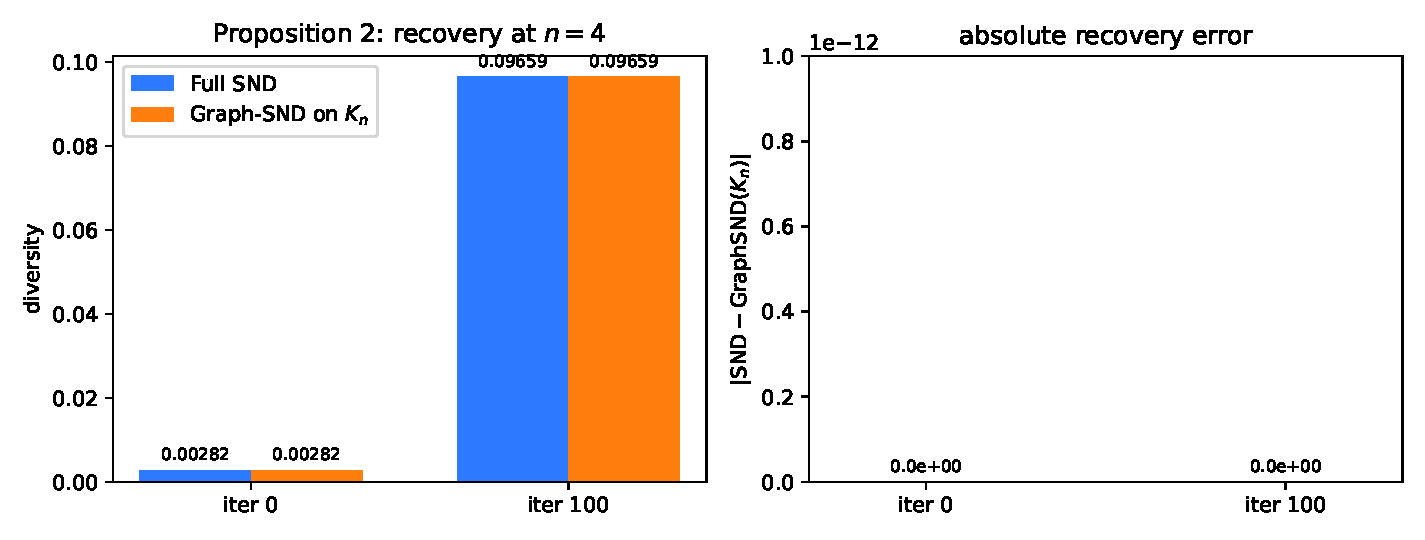
\includegraphics[width=0.85\linewidth]{figures/recovery.pdf}
\caption{Proposition~\ref{prop:recovery}: recovery of $\SND$ by
$\SNDG$ on the complete graph. Left: side-by-side values of $\SND$ and
$\SNDG$ on $K_4$ at iter~0 (near-homogeneous policies) and iter~100
(trained policies). Right: absolute recovery error, which is $0.0$ in
both cases (the y-axis is shown at $10^{-12}$ resolution for context).}
\label{fig:recovery}
\end{figure}

\paragraph{Unbiasedness (Proposition~\ref{prop:unbiased}).} We test
$\E_{G_p}[\widehat{\SND}(G_p)] = \SND(\mathbf{D})$ at $n{=}8$ by
drawing $2{,}000$ independent Bernoulli-$p$ graphs for each
$p \in \{0.1, 0.25, 0.5, 0.75\}$, computing $\widehat{\SND}$ on each,
and reporting the sample mean with a $95\%$ CI
(Figure~\ref{fig:unbiasedness}). The CI contains $\SND(\mathbf{D})$
in every cell across both checkpoints. As a sharper test, the
standardised deviation $|\mathrm{bias}|/\mathrm{SE}$ is approximately
$\mathcal{N}(0,1)$ per cell under an unbiased Gaussian-error
estimator; the maximum observed value across all eight
$(\text{checkpoint}, p)$ cells is $1.42$, well below
$|z_{0.975}| = 1.96$. Estimator variance scales as $1/p$, visible as
widening CIs at small $p$.

\begin{figure}[t]
\centering

\includegraphics[width=0.85\linewidth]{figures/unbiasedness.pdf}
\caption{Proposition~\ref{prop:unbiased}: empirical unbiasedness of
$\widehat{\SND}(G_p)$ at $n=8$. Blue dots and whiskers are the sample
mean and 95\% confidence interval over 2{,}000 random graphs per $p$;
the dashed line is the true $\SND(\mathbf{D})$. Annotations give the
standardized deviation $|\mathrm{bias}|/\mathrm{SE}$, all of which are
well below $1.96$. Left: iter~0 checkpoint. Right: iter~100 checkpoint.}
\label{fig:unbiasedness}
\end{figure}

\paragraph{Concentration (Theorem~\ref{thm:concentration}).} We
evaluate Theorem~\ref{thm:concentration} at $n{=}16$
($|\Pairs|{=}120$) by drawing $2{,}000$ uniform-size edge samples of
each size $m \in \{6, 12, 24, 48, 72, 96\}$ ($5\%$--$80\%$ of all
pairs), computing $\SNDG^{\mathrm{u}}$ on each, and comparing the
empirical distribution of $|\SNDG^{\mathrm{u}} - \SND|$ against theory
at $\delta{=}0.10$ (Figure~\ref{fig:concentration}). Across all $12$
cells, the Hoeffding violation rate is $0.00$---no draw out of
$2{,}000$ exceeds $t_H$---well under the allowed $\delta$; the same
holds for the Serfling refinement of Remark~\ref{rem:serfling}. The
empirical curve sits well below both bounds, as expected for
distribution-free guarantees that are worst-case tight only at
population variance $D_{\max}^2/4$; it still exhibits the predicted
$O(1/\sqrt{m})$ slope on the log-log axis, and Serfling is uniformly
tighter than Hoeffding with the gap widening at large sampling
fractions.

\begin{figure}[t]
\centering
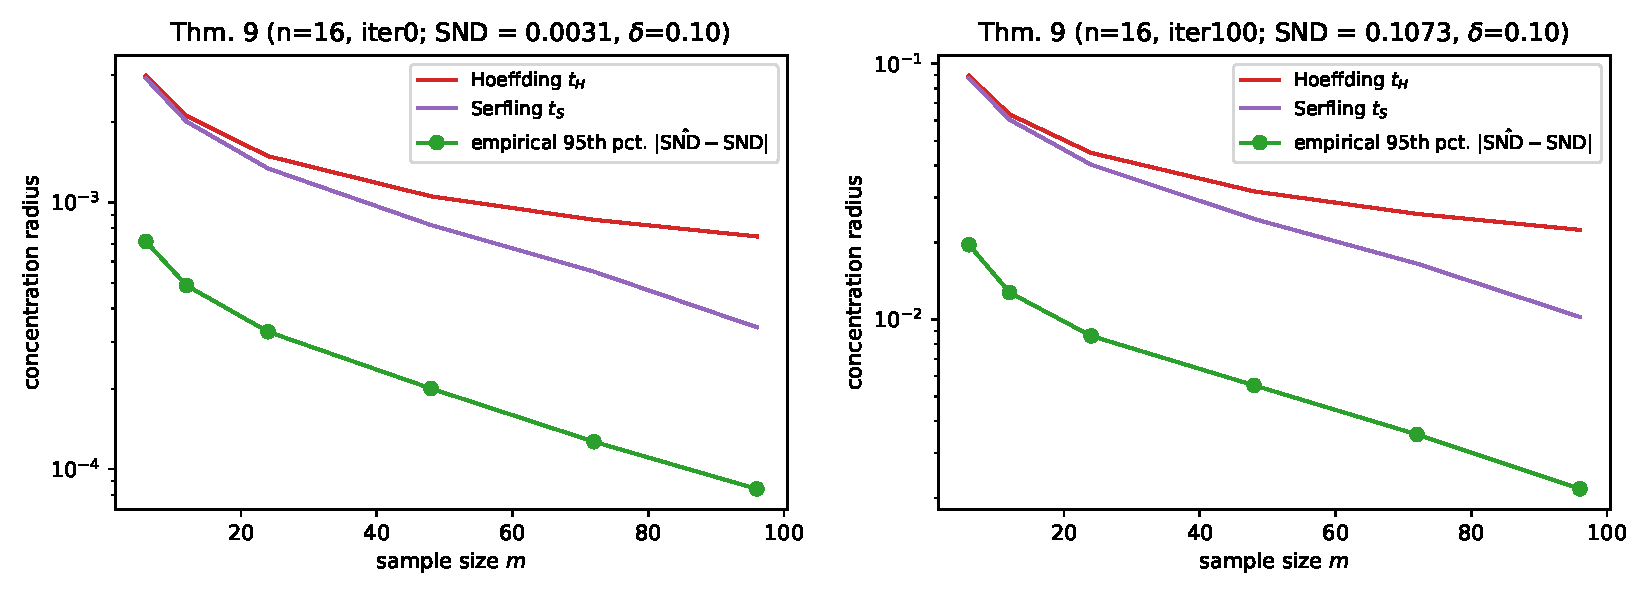
\includegraphics[width=0.85\linewidth]{figures/concentration.pdf}
\caption{Theorem~\ref{thm:concentration}: concentration of
$\SNDG^{\mathrm{u}}$ around $\SND$ at $n=16$. Red: Hoeffding radius
$t_H$ from Theorem~\ref{thm:concentration}. Purple: Serfling radius
$t_S$ from Remark~\ref{rem:serfling}. Green: empirical 95th-percentile
of $|\SNDG^{\mathrm{u}} - \SND|$ over 2{,}000 uniform-size edge
samples per $m$. Both axes are log-scaled. Across all 12 cells, zero
draws violate either bound. The empirical gap reflects the fact that
Hoeffding and Serfling are worst-case over populations bounded in
$[0, D_{\max}]$; the true $d(i,j)$ variance is much smaller.}
\label{fig:concentration}
\end{figure}

\paragraph{CPU wall-clock sweep at $n\in\{4, 8, 16\}$.} As a
pre-condition to the larger-$n$ GPU results reported in
Section~\ref{sec:experiments:timing}, we run the same
$\SNDG$-vs-$\SND$ timing comparison on the iter-$100$ checkpoint
across $n \in \{4, 8, 16\}$ and $p \in \{0.1, 0.25, 0.5, 0.75, 1.0\}$,
$20$ trials per cell, CPU only. Figure~\ref{fig:timing} reports
speedup and absolute times: at $p{=}0.1$ we observe
$10$--$17\times$ speedups across $n$, decaying monotonically to
$\approx 1\times$ at $p{=}1.0$, consistent with the
$\binom{n}{2}/\E[|E(G_p)|]=1/p$ analytical prediction modulo
small-$n$ vectorisation overhead.

\begin{figure}[t]
\centering
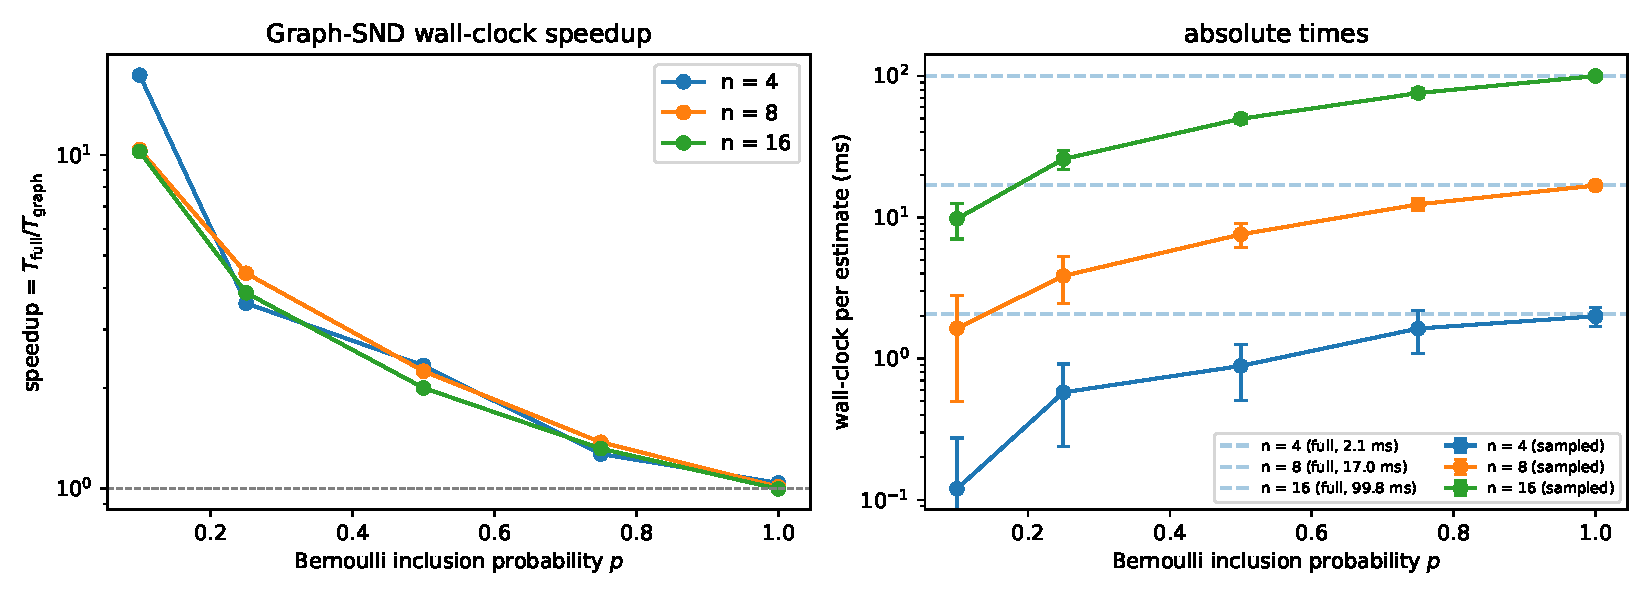
\includegraphics[width=0.85\linewidth]{figures/timing.pdf}
\caption{Proposition~\ref{prop:complexity}: wall-clock scaling of
$\SNDG$ versus $\SND$ (CPU, $n\in\{4,8,16\}$).
Left: speedup $T_{\mathrm{full}} / T_{\mathrm{sampled}}$ against
Bernoulli inclusion probability $p$, one line per team size $n$.
Right: absolute wall-clock time per estimate with error bars over 20
trials. Dashed horizontal lines mark the full-$\SND$ cost at each
$n$; solid lines are the sampled $\SNDG$ cost. The red curve in the
right panel of Figure~\ref{fig:timing-n500} plots the $p=0.1$
speedups reported here.}
\label{fig:timing}
\end{figure}

% ------------------------------------------------------------------
% Appendix: DiCo + Bernoulli-0.1 feasibility at n=50 (one seed).
% Gated on the n=50 feasibility run succeeding. If the run converges,
% flip \hasneurisfiftyresultsfalse -> \hasneurisfiftyresultstrue below
% (one-line change) and rerun the plotter to produce
% figures/neurips_n50_feasibility.pdf. Otherwise the block is a no-op
% and the submission is unchanged.
\newif\ifhasneurisfiftyresults
\hasneurisfiftyresultsfalse
\ifhasneurisfiftyresults
\section{DiCo + Bernoulli-$0.1$ feasibility at $n{=}50$}
\label{app:dico-n50}

Figure~\ref{fig:dico-n50} reports a single-seed feasibility run of DiCo
with Bernoulli-$0.1$ Graph-SND on VMAS Dispersion at $n{=}50$,
alongside a matched diversity-off IPPO baseline at the same team
size. Hyperparameters follow
Section~\ref{sec:experiments:dico-dispersion} except
$\texttt{on\_policy\_n\_envs\_per\_worker}{=}120$ and
$\texttt{on\_policy\_collected\_frames\_per\_batch}{=}12{,}000$
(reduced from $600$ and $60{,}000$ to keep the per-iteration rollout
within a single RTX~4090's memory budget at $5{\times}$ more
per-agent tensors); all other experiment and model settings match
the $n{=}10$ run of Section~\ref{sec:experiments:dico-dispersion}. The
sole purpose of this run is to show that the DiCo closed loop
continues to function when the Bernoulli estimator's expected edge
count $\mathbb{E}[|E(G_{0.1})|]{=}0.1\binom{50}{2}{=}122.5$ is the
sole signal used by the controller; it is a single seed and so is not
a statistical claim, only a feasibility demonstration at
${\approx}5{\times}$ the team size of the main Dispersion experiment.

\begin{figure}[t]
\centering
\includegraphics[width=0.95\linewidth]{figures/neurips_n50_feasibility.pdf}
\caption{Feasibility: DiCo + Bernoulli-$0.1$ Graph-SND on VMAS
Dispersion at $n{=}50$, one seed. \textbf{Blue:} IPPO baseline,
diversity control disabled. \textbf{Red:} DiCo with Bernoulli-$0.1$
Graph-SND, $\SND_{\mathrm{des}}{=}0.1$. Bands on panel~3 are
mean~$\pm$~std (single seed, so equal to the mean); on panels~1 and
2 the bands are the per-iteration rolling-window std. The Bernoulli
Graph-SND run tracks $\SND_{\mathrm{des}}{=}0.1$ and beats the
diversity-off baseline on terminal reward at $n{=}50$, consistent
with the $n{=}10$ multi-seed result of
Figure~\ref{fig:dico-dispersion-knn} but at ${\approx}5{\times}$ the
team size.}
\label{fig:dico-n50}
\end{figure}
\fi

\end{document}